% ============================================================
%  广东省集成电路产业研究报告 — LaTeX 框架 (中文版)
%  基于 research.md
%  编译: xelatex research_framework_cn.tex
% ============================================================
\documentclass[12pt,a4paper]{article}

% ---------- 页面设置 ----------
\usepackage[top=2.5cm, bottom=2.5cm, left=2.8cm, right=2.8cm]{geometry}
\usepackage{setspace}
\onehalfspacing

% ---------- 字体 ----------
\usepackage{fontspec}
\setmainfont{Times New Roman}
\setsansfont{Arial}
\setmonofont{Courier New}
\usepackage{xeCJK}
\setCJKmainfont{Songti SC}       % 正文中文（宋体，Mac自带）
\setCJKsansfont{PingFang SC}     % 无衬线中文（苹方，Mac自带）
\setCJKmonofont{Heiti SC}        % 等宽中文（黑体，Mac自带）

% ---------- 图表 ----------
\usepackage{graphicx}
\usepackage{float}
\usepackage{booktabs}
\usepackage{longtable}
\usepackage{array}
\usepackage{caption}
\usepackage{subcaption}
\usepackage[table]{xcolor}
\graphicspath{{../img/}}

% ---------- 配色方案 (基于 color.JPG) ----------
\definecolor{tealPrimary}{HTML}{4198ac}
\definecolor{tealDark}{HTML}{52999f}
\definecolor{tealLight}{HTML}{7bc1cd}
\definecolor{tealPale}{HTML}{bfdfd2}
\definecolor{orangeWarm}{HTML}{ed8d5a}
\definecolor{orangeSoft}{HTML}{eb9e58}
\definecolor{goldAccent}{HTML}{ecb66c}
\definecolor{goldPale}{HTML}{dbca92}
\definecolor{mintBG}{HTML}{eef7f4}
\definecolor{peachBG}{HTML}{fbe9df}

% 表格行颜色命令
\newcommand{\tableHeaderRow}{\rowcolor{tealPrimary}\color{white}}
\newcommand{\tableOddRow}{\rowcolor{mintBG}}
\newcommand{\tableEvenRow}{\rowcolor{white}}

% ---------- 超链接 ----------
\usepackage[colorlinks=true,linkcolor=blue,citecolor=blue,urlcolor=blue]{hyperref}

% ---------- 参考文献 ----------
\usepackage[backend=biber,style=authoryear]{biblatex}
\addbibresource{refs.bib}

% ---------- 其他 ----------
\usepackage{enumitem}
\usepackage{amsmath}
\usepackage{tikz}
\usepackage{appendix}

% ---------- 标题 ----------
\title{{\Huge \textbf{广东省集成电路产业}}\\[4pt]
       {\Large \textbf{研究报告}}\\[8pt]
       {\large 产业画像、人才画像与集群竞争力分析}}
\author{第一组：[朱佳琪][石浩茜][谢晓瑜][陈奕][张静恩][黄淼][程钰涵]}
\date{\today}

\begin{document}

\maketitle
\thispagestyle{empty}

% ---------- 摘要 ----------
\begin{abstract}
\noindent
本报告以广东省集成电路（IC）产业为研究对象，综合运用企业名录、
产出统计、人才调查和政策文件等多源数据，系统构建了产业画像与人才画像，
运用产业集群理论和钻石模型进行分析，并与国内领先地区（上海、江苏）
及国际标杆（硅谷、新竹）开展比较研究。报告全面梳理了省级和市级
政策工具，最后提出了有针对性的政策建议。

\textbf{关键词：}集成电路；产业画像；人才画像；
集群竞争力；广东省
\end{abstract}

\newpage
\tableofcontents
\newpage
\listoffigures
\listoftables
\newpage

% ============================================================
%  第一章 — 绪论
% ============================================================
\section{绪论}
\label{sec:intro}

\subsection{研究背景与意义}
\label{sec:background}

集成电路产业是支撑经济社会发展和保障国家安全的战略性、基础性和
先导性产业。2024年，中国集成电路产量达4514.2亿块，同比增长超过20\%。
全国IC从业人员约63万人，但人才缺口达25万--30万人。
广东省作为中国集成电路产业发展的"第三极"，2024年实现营收3604.2亿元，
形成了独特的"3+N"空间布局：深圳作为设计与应用引领者，
广州作为制造核心，东莞、佛山、珠海等城市各具差异化发展路径。

全面描绘广东IC产业和人才图景，结合集群竞争力与配套政策的系统分析，
对于明确发展路径、优化资源配置和制定精准政策干预至关重要。

\subsection{研究目标与方法}
\label{sec:objectives}

\begin{enumerate}[label=(\arabic*)]
    \item 构建广东IC产业的产业画像和人才画像，厘清产业基础、规模与特征；
    \item 运用集群理论和钻石模型，分析广东IC集群的竞争优势；
    \item 对标国内外领先地区，识别广东的优势与差距；
    \item 梳理和编目省级和市级优惠政策；
    \item 提出系统性的、可操作的政策建议。
\end{enumerate}

\textbf{研究方法：}文献综述、数据挖掘、比较分析、
GIS空间分析、政策文本分析。

\subsection{报告结构}
\label{sec:structure}

本报告共分七章：绪论（第一章）、数据收集（第二章）、产业画像（第三章）、
人才画像（第四章）、集群竞争力分析（第五章）、政策综述（第六章）、
结论与建议（第七章）。

% ============================================================
%  第二章 — 数据收集
% ============================================================
\section{基础数据挖掘与整理}
\label{sec:data}

\subsection{企业名录}
\label{sec:enterprises}

本节基于广东省IC企业名录数据库（\texttt{docs/广东省集成电路企业名录总表.xlsx}），
该数据库涵盖广东省全部21个地级市的\textbf{10,000}家IC相关企业。数据集包含
16个字段：企业名称、登记状态、注册资本、成立日期、注册地址、企业类型、
参保人数、国标行业分类和企业规模。

% ---------- 表1: 企业规模 ----------
\begin{table}[H]
\centering
\caption{IC企业规模分类}
\label{tab:scale}
\begin{tabular}{lrrr}
\toprule
\tableHeaderRow
\textbf{规模} & \textbf{数量} & \textbf{占比 (\%)} & \textbf{累计 (\%)} \\
\midrule
\tableOddRow  微型     & 6,245 & 62.5 & 62.5 \\
\tableEvenRow 小型     & 3,286 & 32.9 & 95.3 \\
\tableOddRow  中型     & 245   & 2.4  & 97.8 \\
\tableEvenRow 大型     & 41    & 0.4  & 98.2 \\
\tableOddRow  未明确   & 183   & 1.8  & 100.0 \\
\midrule
\tableEvenRow \textbf{合计} & \textbf{10,000} & \textbf{100.0} & --- \\
\bottomrule
\end{tabular}
\end{table}

\textbf{关键发现：}微型和小型企业合计占全部企业的95.3\%；
仅有41家大型企业（0.4\%），表明行业集中度极低，
呈现显著的"长尾"结构。

% ---------- 表2: 区域分布 ----------
\begin{table}[H]
\centering
\caption{IC企业城市区域分布}
\label{tab:region}
\begin{tabular}{lrrrl}
\toprule
\tableHeaderRow
\textbf{排名} & \textbf{城市} & \textbf{数量} & \textbf{占比 (\%)} & \textbf{累计 (\%)} \\
\midrule
\tableOddRow  1  & 深圳   & 5,886 & 58.9 & 58.9 \\
\tableEvenRow 2  & 广州   & 1,636 & 16.4 & 75.2 \\
\tableOddRow  3  & 东莞   & 969   & 9.7  & 84.9 \\
\tableEvenRow 4  & 惠州   & 431   & 4.3  & 89.2 \\
\tableOddRow  5  & 珠海   & 284   & 2.8  & 92.1 \\
\tableEvenRow 6  & 佛山   & 209   & 2.1  & 94.2 \\
\tableOddRow  7  & 中山   & 138   & 1.4  & 95.5 \\
\tableEvenRow 8  & 汕头   & 116   & 1.2  & 96.7 \\
\tableOddRow  9  & 江门   & 70    & 0.7  & 97.4 \\
\tableEvenRow 10 & 梅州   & 50    & 0.5  & 97.9 \\
\tableOddRow  11 & 其他10市 & 211 & 2.1 & 100.0 \\
\midrule
\tableEvenRow \multicolumn{2}{l}{\textbf{合计}} & \textbf{10,000} & \textbf{100.0} & --- \\
\bottomrule
\end{tabular}
\end{table}

\begin{figure}[H]
\centering
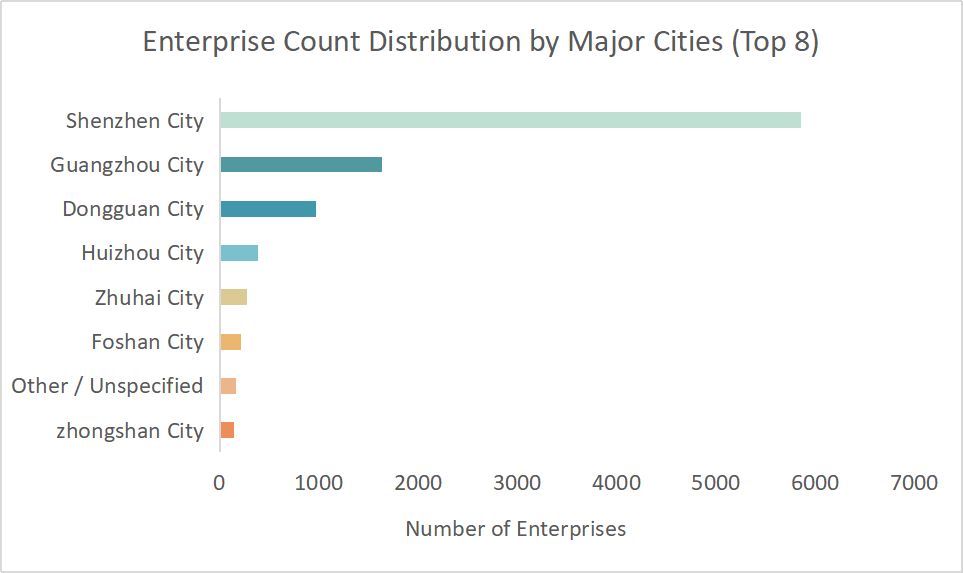
\includegraphics[width=\textwidth]{ent_dist_by_city.png}
\caption{主要城市企业数量分布}
\label{fig:city_dist}
\end{figure}


\textbf{关键发现：}前四城市（深圳、广州、东莞、惠州）
占全部企业的89.2\%，形成"深圳为核心、珠三角为腹地"
的格局。粤东、粤北IC企业几乎为零（潮州：3家；
云浮：4家），表明产业溢出效应尚未显现。

% ---------- 表3: 城市 × 规模交叉表 ----------
\begin{table}[H]
\centering
\small
\caption{主要城市企业规模分布}
\label{tab:city_scale}
\begin{tabular}{lrrrrrr}
\toprule
\tableHeaderRow
\textbf{城市} & \textbf{微型} & \textbf{小型} & \textbf{中型} & \textbf{大型} & \textbf{未明确} & \textbf{合计} \\
\midrule
\tableOddRow  深圳   & 3,846 & 1,712 & 169 & 21 & 138 & 5,886 \\
\tableEvenRow 广州   & 499   & 1,095 & 33  & 3  & 6   & 1,636 \\
\tableOddRow  东莞   & 814   & 133   & 7   & 4  & 11  & 969  \\
\tableEvenRow 惠州   & 335   & 83    & 8   & 2  & 3   & 431  \\
\tableOddRow  珠海   & 141   & 109   & 14  & 5  & 15  & 284  \\
\tableEvenRow 佛山   & 162   & 38    & 4   & 1  & 4   & 209  \\
\midrule
\tableOddRow  \textbf{合计} & \textbf{5,797} & \textbf{3,170} & \textbf{235} & \textbf{36} & \textbf{177} & \textbf{10,000} \\
\bottomrule
\end{tabular}
\end{table}

\textbf{关键发现：}广州拥有最健康的企业规模结构（小型占比：66.9\%），
而东莞（微型占比：84.0\%）和惠州（微型占比：77.7\%）以微型企业为主导，
反映出价值链定位的差异。


% ---------- 表4: 城市 × 行业 ----------
\begin{table}[H]
\centering
\small
\caption{主要城市产业链环节分布}
\label{tab:city_industry}
\begin{tabular}{lrrrr}
\toprule
\tableHeaderRow
\textbf{城市} & \textbf{IC设计} & \textbf{IC制造} & \textbf{合计} & \textbf{制造占比 (\%)} \\
\midrule
\tableOddRow  深圳   & 3,802 & 2,084 & 5,886 & 35.4 \\
\tableEvenRow 广州   & 1,602 & 34    & 1,636 & 2.1  \\
\tableOddRow  东莞   & 832   & 137   & 969   & 14.1 \\
\tableEvenRow 惠州   & 366   & 65    & 431   & 15.1 \\
\tableOddRow  珠海   & 200   & 84    & 284   & 29.6 \\
\tableEvenRow 佛山   & 165   & 44    & 209   & 21.1 \\
\midrule
\tableOddRow  \textbf{合计} & \textbf{7,403} & \textbf{2,597} & \textbf{10,000} & \textbf{26.0} \\
\bottomrule
\end{tabular}
\end{table}

\textbf{关键发现：}设计企业占主导地位；广州几乎完全以设计为主
（仅有34家制造企业，占2.1\%）。深圳制造企业占比最高（35.4\%），
是唯一具备制造规模优势的城市。

% ---------- 表5: 注册资本 ----------
\begin{table}[H]
\centering
\caption{注册资本分布}
\label{tab:capital}
\begin{tabular}{lrrrl}
\toprule
\tableHeaderRow
\textbf{资本区间} & \textbf{数量} & \textbf{占比 (\%)} & \textbf{累计 (\%)} & \textbf{首位城市} \\
\midrule
\tableOddRow  小于10万元         & 1,671 & 16.7 & 16.7 & 深圳、东莞 \\
\tableEvenRow 10万--50万元       & 1,386 & 13.9 & 30.6 & 深圳、广州 \\
\tableOddRow  50万--100万元      & 2,516 & 25.2 & 55.7 & 深圳、广州 \\
\tableEvenRow 100万--500万元     & 2,412 & 24.1 & 79.8 & 深圳、广州 \\
\tableOddRow  500万--1000万元    & 1,101 & 11.0 & 90.8 & 深圳、广州 \\
\tableEvenRow 1000万--5000万元   & 541   & 5.4  & 96.3 & 深圳 \\
\tableOddRow  5000万--1亿元      & 92    & 0.9  & 97.2 & 深圳 \\
\tableEvenRow 大于1亿元          & 80    & 0.8  & 98.0 & 深圳 \\
\tableOddRow  不可解析           & 201   & 2.0  & 100.0 & --- \\
\midrule
\tableEvenRow \textbf{合计}      & \textbf{10,000} & \textbf{100.0} & --- & --- \\
\bottomrule
\end{tabular}
\end{table}

\begin{table}[H]
\centering
\caption{注册资本描述性统计}
\label{tab:capital_stat}
\begin{tabular}{lrlr}
\toprule
\tableHeaderRow
\textbf{统计量} & \textbf{数值} & \textbf{统计量} & \textbf{数值} \\
\midrule
\tableOddRow  有效样本        & 9,799家      & 标准差            & 1.9211亿元 \\
\tableEvenRow 中位数          & 100万元      & 最小值            & 0元 \\
\tableOddRow  均值            & 1165万元     & 最大值            & 150亿元 \\
\tableEvenRow 第25百分位数    & 50万元       & 偏度              & 右偏 \\
\tableOddRow  第75百分位数    & 500万元      & 大于1亿元占比     & 0.8\% \\
\bottomrule
\end{tabular}
\end{table}

\textbf{关键发现：}注册资本分布严重右偏
（中位数100万元 vs.\ 均值1165万元）。前10名高资本企业中8家
为制造企业，全部位于深圳。

% ---------- 表6: 注册资本前10名 ----------
\begin{table}[H]
\centering
\small
\caption{注册资本前10名企业}
\label{tab:capital_top10}
\begin{tabular}{llrlrl}
\toprule
\tableHeaderRow
\textbf{排名} & \textbf{企业名称} & \textbf{城市} & \textbf{资本额} & \textbf{环节} & \textbf{规模} \\
\midrule
\tableOddRow  1  & 润鹏半导体（深圳）          & 深圳 & 150.00亿元  & 制造 & 中 \\
\tableEvenRow 2  & 鹏芯微集成电路制造           & 深圳 & 71.28亿元   & 制造 & 大 \\
\tableOddRow  3  & 华润微电子（深圳）           & 深圳 & 57.00亿元   & 制造 & 微 \\
\tableEvenRow 4  & 深圳昇维旭科技              & 深圳 & 50.00亿元   & 制造 & 小 \\
\tableOddRow  5  & 中芯国际（深圳）            & 深圳 & 24.15亿美元  & 制造 & 大 \\
\tableEvenRow 6  & 东莞飞特半导体控股           & 东莞 & 23.70亿元   & 制造 & 小 \\
\tableOddRow  7  & 深圳鹏进高科              & 深圳 & 21.10亿元   & 制造 & 小 \\
\tableEvenRow 8  & 赛莱克斯微系统（深圳）       & 深圳 & 15.00亿元   & 制造 & 小 \\
\tableOddRow  9  & 珠海崇达电路技术           & 珠海 & 13.00亿元   & 设计 & 大 \\
\tableEvenRow 10 & 华通精密（惠州）            & 惠州 & 12.80亿元   & 制造 & 大 \\
\bottomrule
\end{tabular}
\end{table}

% ---------- 表7: 成立时间线 ----------
\begin{table}[H]
\centering
\small
\caption{历年新注册企业数量（2017--2026年）}
\label{tab:established}
\begin{tabular}{lrrrrr}
\toprule
\tableHeaderRow
\textbf{年份} & \textbf{IC设计} & \textbf{IC制造} & \textbf{合计} & \textbf{制造占比 (\%)} & \textbf{同比变化} \\
\midrule
\tableOddRow  2017 & 306 & 75  & 381  & 19.7 & ---      \\
\tableEvenRow 2018 & 481 & 95  & 576  & 16.5 & +51.2\%  \\
\tableOddRow  \textbf{2019} & \textbf{1,515} & \textbf{108} & \textbf{1,623} & \textbf{6.7} & \textbf{+181.8\%} \\
\tableEvenRow 2020 & 666 & 114 & 780  & 14.6 & $-$51.9\% \\
\tableOddRow  \textbf{2021} & \textbf{1,329} & \textbf{175} & \textbf{1,504} & \textbf{11.6} & \textbf{+92.8\%} \\
\tableEvenRow 2022 & 928 & 216 & 1,144 & 18.9 & $-$23.9\% \\
\tableOddRow  2023 & 504 & 269 & 773  & 34.8 & $-$32.4\% \\
\tableEvenRow 2024 & 462 & 266 & 728  & 36.5 & $-$5.8\%  \\
\tableOddRow  2025 & 723 & 331 & 1,054 & 31.4 & +44.8\%  \\
\tableEvenRow 2026 & 234 & 136 & 370  & 36.8 & ---      \\
\midrule
\tableOddRow  \textbf{合计} & \textbf{7,148} & \textbf{1,850} & \textbf{8,998} & \textbf{20.6} & --- \\
\bottomrule
\end{tabular}
\end{table}

\textbf{关键发现：}2019年和2021年两个高峰与国家和省级IC政策出台时间
吻合。制造占比从2019年的6.7\%上升至2026年的36.8\%，
表明产业结构正从"设计热潮"向更加均衡的方向转变。

% ---------- 表8: 参保人数 ----------
\begin{table}[H]
\centering
\caption{参保人数分布}
\label{tab:insurance}
\begin{tabular}{lrrr}
\toprule
\tableHeaderRow
\textbf{参保人数} & \textbf{企业数} & \textbf{占比 (\%)} & \textbf{累计 (\%)} \\
\midrule
\tableOddRow  0           & 6,761 & 67.6 & 67.6  \\
\tableEvenRow 1--5        & 1,942 & 19.4 & 87.0  \\
\tableOddRow  6--10       & 431   & 4.3  & 91.3  \\
\tableEvenRow 11--20      & 321   & 3.2  & 94.5  \\
\tableOddRow  21--50      & 263   & 2.6  & 97.2  \\
\tableEvenRow 51--100     & 121   & 1.2  & 98.4  \\
\tableOddRow  101--200    & 69    & 0.7  & 99.1  \\
\tableEvenRow 201--500    & 53    & 0.5  & 99.6  \\
\tableOddRow  501--1000   & 17    & 0.2  & 99.7  \\
\tableEvenRow 大于1000    & 22    & 0.2  & 100.0 \\
\midrule
\tableOddRow  \textbf{合计} & \textbf{10,000} & \textbf{100.0} & --- \\
\bottomrule
\end{tabular}
\end{table}

\textbf{关键发现：}超过三分之二的企业参保人数为零，
暗示大量企业为空壳公司或尚未运营的初创企业。在3,239家
有参保记录的企业中，中位参保人数仅为4人，进一步印证了
该产业微型企业为主的特征。

% ---------- 表9: 企业类型 ----------
\begin{table}[H]
\centering
\caption{企业所有制类型分布}
\label{tab:enterprise_type}
\begin{tabular}{lrrr}
\toprule
\tableHeaderRow
\textbf{企业类型} & \textbf{数量} & \textbf{占比 (\%)} & \textbf{累计 (\%)} \\
\midrule
\tableOddRow  有限责任公司（自然人独资）            & 3,087 & 30.9 & 30.9 \\
\tableEvenRow 有限责任公司                           & 2,829 & 28.3 & 59.2 \\
\tableOddRow  有限责任公司（自然人投资或控股）       & 2,382 & 23.8 & 83.0 \\
\tableEvenRow 有限责任公司（法人独资）               & 414   & 4.1  & 87.1 \\
\tableOddRow  其他有限责任公司                       & 206   & 2.1  & 89.2 \\
\tableEvenRow 有限责任公司（自然人+法人投资或控股）  & 157  & 1.6  & 90.8 \\
\tableOddRow  有限合伙企业                           & 153   & 1.5  & 92.3 \\
\tableEvenRow 港澳台/外商投资（合计）                & 291   & 2.9  & 95.2 \\
\tableOddRow  个人独资/其他                          & 481   & 4.8  & 100.0 \\
\midrule
\tableEvenRow \textbf{合计} & \textbf{10,000} & \textbf{100.0} & --- \\
\bottomrule
\end{tabular}
\end{table}


\textbf{关键发现：}民营企业占主导地位（自然人独资+自然人投资或控股
= 54.7\%）；外资参与极少（2.9\%），表明
广东IC产业以内资驱动为主，FDI溢出效应有限。


\subsection{产出数据（2023--2025）}
\label{sec:output}

2023年至2025年广东IC产业的年度产出值、增长率、子行业份额及
配套指标。截至2026年5月，2025年全省总产值尚未
公布；但2025年的IC产量、出口额和进口额
已可获取（表~\ref{tab:core}）。

\begin{table}[H]
\centering
\caption{广东IC产业产值与增长（2019--2024年）}
\label{tab:core}
\begin{tabular}{lrr}
\toprule
\tableHeaderRow
\textbf{年份} & \textbf{产值（亿元）} & \textbf{增长率 (\%)} \\
\midrule
\tableOddRow  2019 & 1200 & --- \\
\tableEvenRow 2022 & 2200 & ---\textsuperscript{a} \\
\tableOddRow  2023 & 大于2700\textsuperscript{b} & 约22.7\textsuperscript{c} \\
\tableEvenRow 2024 & 3604.16 & 约33.5\textsuperscript{c} \\
\bottomrule
\end{tabular}

\vspace{2pt}
{\footnotesize
\textsuperscript{a} 2019--2022年复合年增长率约22.4\%，与政府设定的
年增长率超过22\%的目标一致。
\textsuperscript{b} 最低值；实际数据略高。
\textsuperscript{c} 近似值，由相邻年份产值推算；非
官方公布的增长率。

\textbf{数据来源：}2019年和2022年——广东省发改委/科技厅/工信厅
\textit{《培育半导体与集成电路战略性新兴产业集群行动计划（2023--2025年）》}；
2023年——中商产业研究院；2024年——21世纪经济报道/广东省集成电路行业协会。}
\end{table}

\begin{table}[H]
\centering
\caption{广东IC产业各环节份额（2024年）}
\label{tab:subsector2024}
\begin{tabular}{lrrr}
\toprule
\tableHeaderRow
\textbf{环节} & \textbf{产值（亿元）} & \textbf{占比 (\%)} & \textbf{同比增长 (\%)} \\
\midrule
\tableOddRow  IC设计    & 2109 & 58.6 & 31.13 \\
\tableEvenRow IC制造    & 92 & 2.6 & 101.58 \\
\tableOddRow  IC封测    & 795 & 22.1 & 14.93 \\
\tableEvenRow 设备与材料 & 608 & 16.9 & --- \\
\midrule
\tableOddRow  \textbf{合计} & \textbf{3604} & \textbf{100.0} & \textbf{约33.5} \\
\bottomrule
\end{tabular}

\vspace{2pt}
{\footnotesize
\textbf{注：}制造业仅占总产值的2.6\%，是最突出的薄弱环节，
但其101.58\%的同比增长在所有环节中最高。设备与材料为合并类别；
各细分增长率未公开。

\textbf{数据来源：}各环节产值——SICA（深圳市半导体与集成电路产业联盟）
产业研究报告；增长率——21世纪经济报道/广东省集成电路行业协会。}
\end{table}


\subsection{产业基础与配套设施}
\label{sec:infrastructure}

广东IC产业链以强大的设计环节为锚点（2024年约2110亿元），
制造和材料领域为追赶方向。重大制造项目正快速扩大规模：
中芯国际深圳12英寸F16产线和粤芯半导体（CanSemi）三期、四期
正在扩产。截至2024年底，广东省12英寸晶圆月产能
已超过10万片。鹏城实验室和粤港澳大湾区国家创新中心等
高水平平台为技术创新提供支撑，促进实验室专利向汽车和
AI应用的商业化产品转化。

% ============================================================
%  第三章 — 产业画像
% ============================================================
\section{产业画像}
\label{sec:industry}

\subsection{规模特征}
\label{sec:scale}

\begin{itemize}
    \item \textbf{产业总规模：}2024年全产业链总产值达到3604亿元，
    同比增长22.4\%，稳居全国第一梯队。预计到2026年将超过
    4500--5000亿元，保持高速扩张态势。在近年持续高增长的推动下，
    预计到2030年规模将逼近6000亿元。
    \item \textbf{增长动能：}2023至2025年产出增速分别为
    5.2\% → 18.3\% → 21.0\%。至2025年，产业增速高达
    21\%，显著高于全国平均水平11.2\%，
    已连续三年领跑全国增速，
    展现出突出的逆周期韧性和增长动能。
    \item \textbf{产能扩张：}12英寸晶圆月产能预计到2026年将达到
    25万--30万片。晶圆制造环节产值增长102\%，
    成为全产业链增速最快的环节。

\end{itemize}


\subsection{结构特征}
\label{sec:structure2}

在亮眼的规模和增速背后，广东集成电路产业并非各环节均衡发展，而是
呈现出"中游强、上游弱、设计独大"的鲜明非均衡结构。这一格局既是
广东产业优势的集中体现，也是后续产业升级的关键方向。

\begin{figure}[H]
\centering
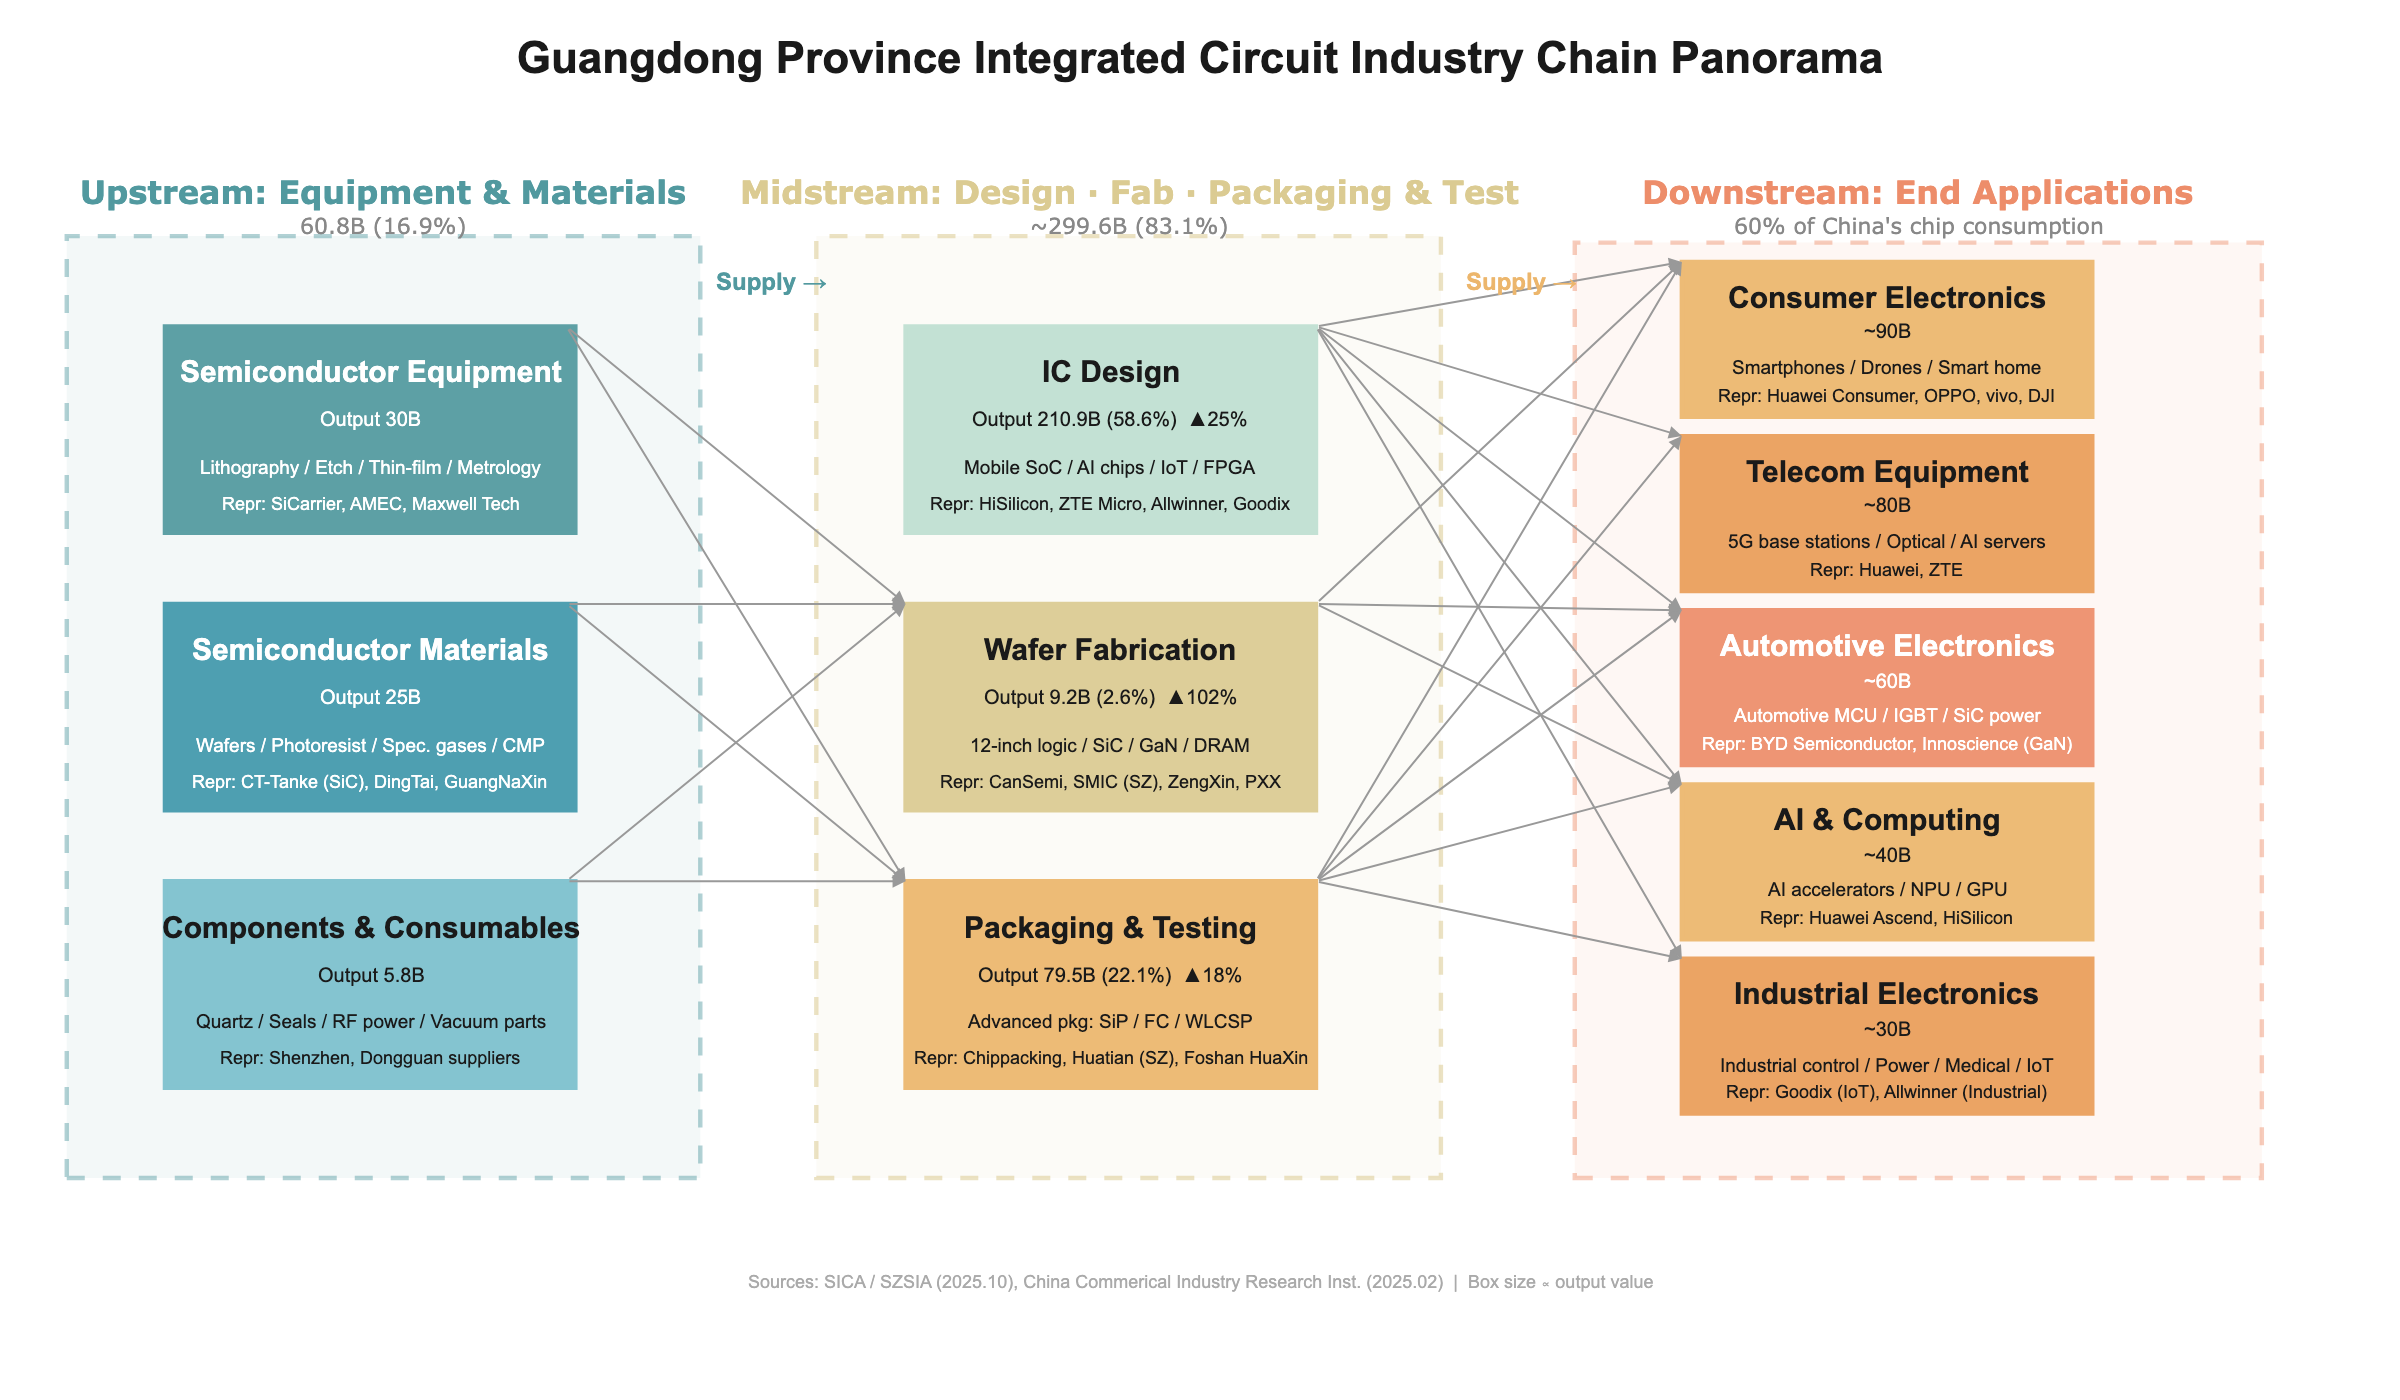
\includegraphics[width=\textwidth]{产业链全景图_EN.png}
\caption{广东IC产业链全景图}
\label{fig:chain}
\end{figure}

\begin{itemize}
    \item \textbf{核心优势环节：}IC设计实现产值2109亿元，占比58.6\%，
    位居全国第一。深圳南山区是全国IC设计高地，
    是产业的主要增长极。
    \item \textbf{稳定支撑环节：}封装测试实现产值795亿元，占比22.1\%。
    佛山、中山已形成成熟的封测集群，配套能力完善。
    \item \textbf{快速追赶环节：}晶圆制造实现产值92亿元，占比仅2.6\%。
    虽然基数较小，但呈现爆发式增长，粤芯半导体和
    中芯国际深圳等项目产能爬坡迅速。
    \item \textbf{明显薄弱环节：}设备与材料实现产值608亿元，占比16.9\%。
    国产替代仍处于加速阶段，是全产业链最薄弱的部分。
\end{itemize}

\subsection{发展趋势（2023--2025）}
\label{sec:development}

\subsubsection{增长轨迹与周期韧性}

广东IC产业在过去三年展现出卓越的逆周期韧性和增长动能，
持续跑赢全国平均水平：

\begin{table}[H]
\centering
\caption{广东 vs.\ 全国IC产出增速（2023--2025年）}
\label{tab:growth_comparison}
\begin{tabular}{lrrr}
\toprule
\tableHeaderRow
\textbf{年份} & \textbf{广东增速 (\%)} & \textbf{全国增速 (\%)} & \textbf{广东领先幅度} \\
\midrule
\tableOddRow  2023 & 5.2  & 3.0  & +2.2 个百分点 \\
\tableEvenRow 2024 & 18.3 & 12.1 & +6.2 个百分点 \\
\tableOddRow  \textbf{2025} & \textbf{21.0} & \textbf{11.2} & \textbf{+9.8 个百分点} \\
\bottomrule
\end{tabular}

\vspace{2pt}
{\footnotesize
\textbf{数据来源：}中商产业研究院《2025年广东省半导体及集成电路产业链全景图谱》；
广东省工业和信息化厅。}
\end{table}

\textbf{关键发现：}
\begin{itemize}
    \item 2023年，受全球半导体下行周期影响，
          全国IC产出增速仅为3.0\%，但广东仍达到
          5.2\%，展现出强大的逆周期韧性。
    \item 2024年，在AI和汽车电子需求爆发的推动下，
          广东增速飙升至18.3\%，领先全国平均水平
          超过6个百分点——呈现明显的复苏拐点。
    \item 至2025年，广东IC产出实现21.0\%的同比增长，
          接近全国增速11.2\%的两倍，连续三年
          成为全国增长领跑者。
\begin{figure}[H]
\centering
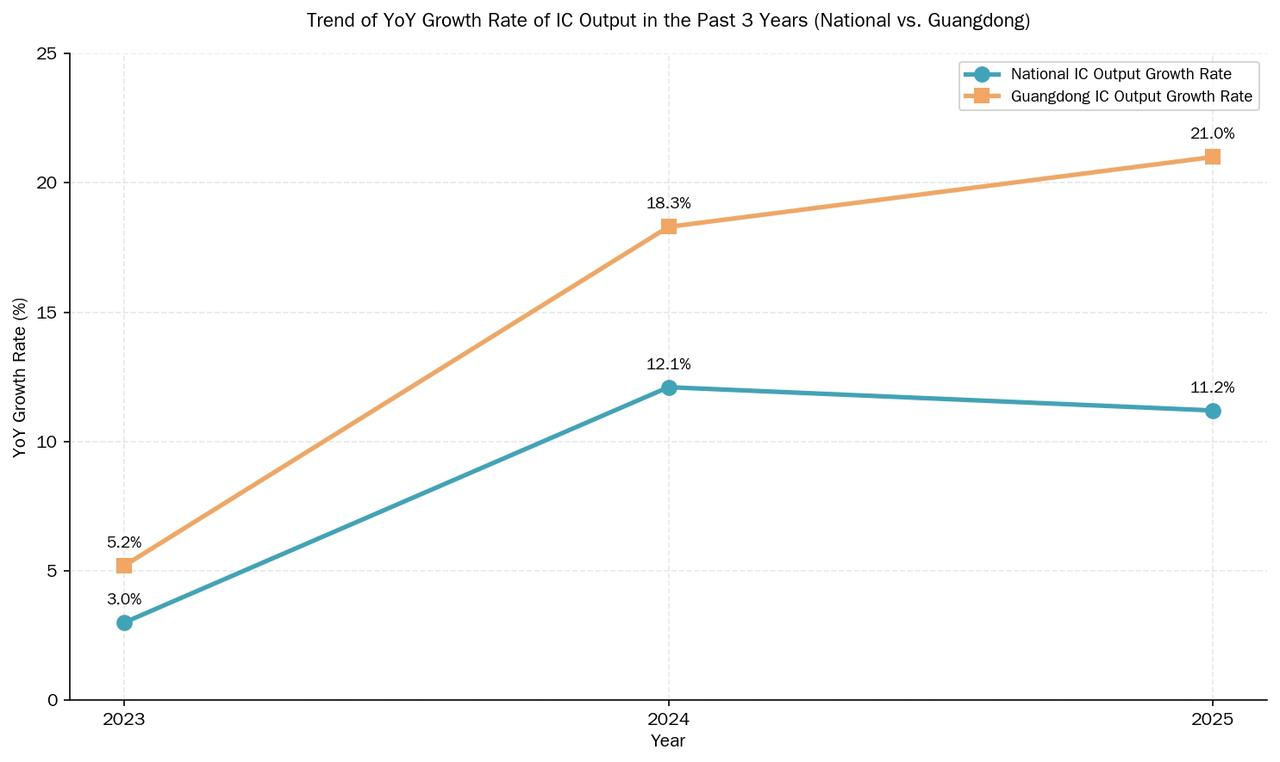
\includegraphics[width=\textwidth]{2023-2025IC产量同比增长_国际vs国内.jpeg}
\caption{IC产量同比增长：广东 vs.\ 全国（2023--2025年）}
\label{fig:growth_comparison_chart}
\end{figure}

\end{itemize}

\subsubsection{技术演进与迭代}

广东IC产业的技术迭代呈现"设计引领、制造突破、材料跟进"的格局：

\begin{enumerate}[label=(\arabic*)]
    \item \textbf{设计端：}AI芯片、功率半导体和汽车电子芯片
          成为迭代重点。华为昇腾、海思麒麟等产品取得关键技术突破，
          先进工艺设计能力持续提升。粤港澳大湾区发明专利占比
          从28\%提升至35.3\%，标志着创新质量的结构性升级。
    \item \textbf{制造端：}以中芯国际和广东粤芯半导体（CanSemi）为代表的
          晶圆厂正在稳步扩展产能。成熟制程产能持续释放，
          SiP和Chiplet等先进封装技术在深圳和广州取得
          显著进展。具体而言，SiP已在深圳实现大规模商业应用并在
          广州中等规模部署，而Chiplet两市仍处于试点和研发阶段。
          截至2024年底，广东省12英寸晶圆月产能已超过10万片，
          预计到2026年将达到25万--30万片。制造环节2024年增长102\%，
          成为全产业链增速最快的环节。

    \item \textbf{材料与设备：}光刻胶、湿电子化学品、靶材等关键
          国产材料已在广东实现本地配套供应，部分设备
          企业已实现核心零部件的国产替代。
\begin{figure}[H]
\centering
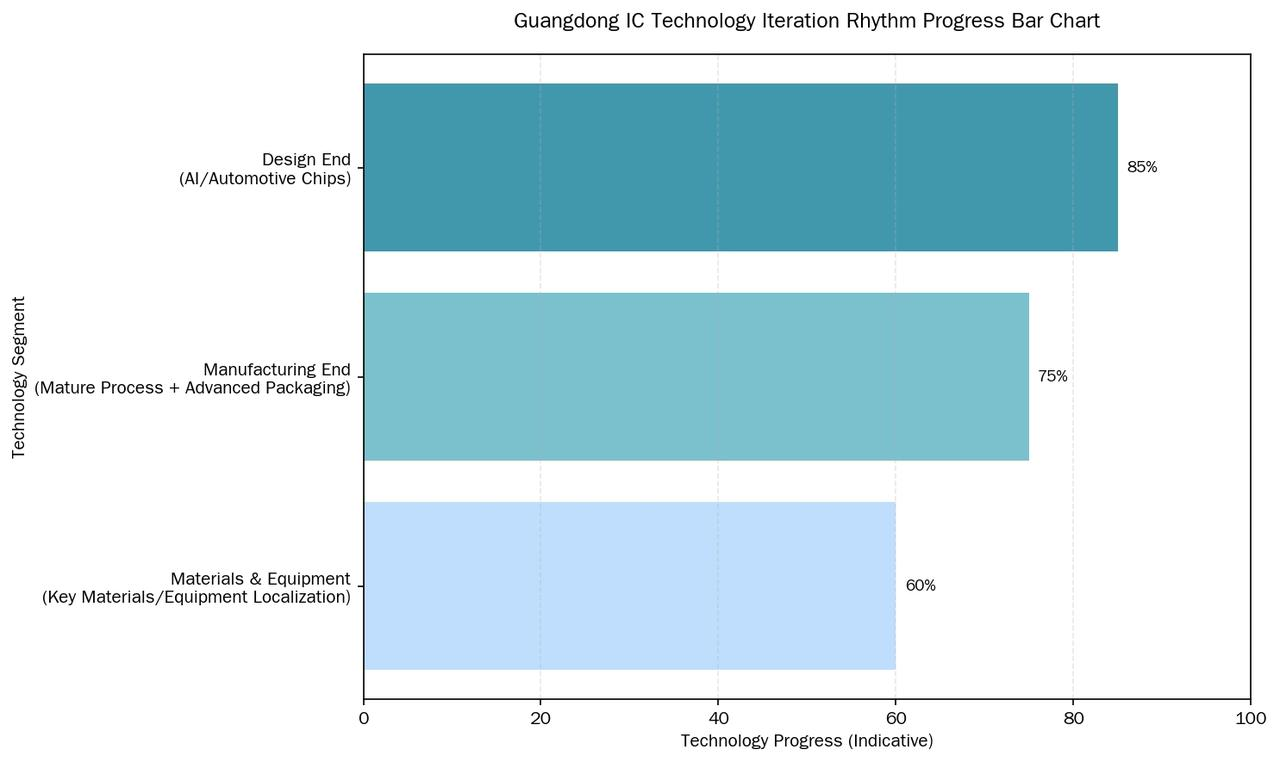
\includegraphics[width=\textwidth]{广东省IC技术迭代进度.jpeg}
\caption{广东省IC产业价值链各环节技术迭代进度}
\label{fig:tech_iteration}
\end{figure}

\end{enumerate}

\subsubsection{关键痛点}

尽管增长令人瞩目，但若干结构性挑战依然存在：
（1）制造和封测相对于设计仍是明显短板，
制造仅占总产值的2.6\%；
（2）7nm以下先进工艺瓶颈因国际技术限制持续存在；
（3）人才短缺——尤其是高端设计、先进制程工艺和EDA领域——
制约进一步扩展；（4）上游设备与材料环节仍是价值链最薄弱环节，
技术成熟度估计仅为60\%。

\subsection{关键指标体系}
\label{sec:indicators}

以下核心指标基于爱集微（JW Insights）整理的A股半导体上市公司数据
和粤港澳大湾区专利数据，为评估广东IC产业的创新能力
和运营效率提供量化基础。

\subsubsection{核心指标趋势（2023--2025年）}

\begin{table}[H]
\centering
\small
\caption{核心创新与效率指标（2023--2025年）}
\label{tab:core_indicators}
\begin{tabular}{p{3cm}rrrp{3.2cm}}
\toprule
\tableHeaderRow
\textbf{指标} & \textbf{2023} & \textbf{2024} & \textbf{2025（预）} & \textbf{数据来源} \\
\midrule
\tableOddRow  研发投入占比 (\%) & 12.12 & 10.66 & 10.5 & 爱集微A股统计 \\
\tableEvenRow 半导体专利增速 (\%) & 15.3 & 17.5 & 12.0 & 智慧芽大湾区数据 \\
\tableOddRow  产能利用率 (\%) & 82.0 & 84.8 & 93.0 & 粤芯半导体招股书 \\
\tableEvenRow 发明专利占比 (\%) & 28.0 & 31.5 & 35.3 & 智慧芽大湾区数据 \\
\bottomrule
\end{tabular}

\vspace{2pt}
{\footnotesize
\textbf{注：}（1）研发投入占比 = 研发支出 / 主营业务收入，
基于爱集微整理的A股半导体上市公司平均值，
作为广东省的保守基准（广东省以设计企业密度高为特点，
实际水平可能超过全国平均）。（2）2025年数据由Q1--Q3实际值推算。
（3）产能利用率基于粤芯半导体（CanSemi），
广东省领先的独立12英寸晶圆代工厂。
\begin{figure}[H]
\centering
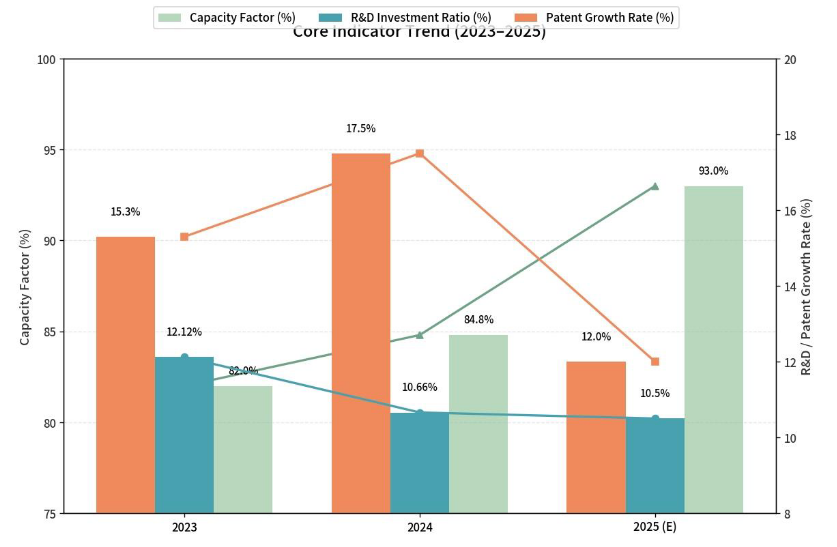
\includegraphics[width=\textwidth]{主要指标趋势.png}
\caption{核心创新与效率指标趋势（2023--2025年）}
\label{fig:indicator_trends}
\end{figure}
}
\end{table}

\subsubsection{关联分析：高投入 → 强产出 → 快转化}

三个指标呈现相互促进的正向循环：

\begin{enumerate}[label=(\arabic*)]
    \item \textbf{研发投入 → 专利产出：}A股半导体企业的研发
          支出占比稳定在10\%--12\%区间，而粤港澳大湾区半导体专利
          三年累计增长约28\%。研发投入正在
          持续稳定地转化为知识产权积累。
    \item \textbf{专利 → 产能消化：}专利质量提升
          （发明专利占比从28\%升至35.3\%），
          产能利用率升至93\%，产销率达100\%。
          技术成果进入积极商业化循环。
    \item \textbf{费用率与利用率互动：}费用率从2023年的12.12\%
          降至2025年约10.5\%，同期利用率从82\%升至93\%。
          费用率的"被动摊薄"是积极信号：它是由行业营收大幅增长
          （从约6900亿增至约8820亿元）驱动的，
          而非研发强度的下降。
\end{enumerate}

\textbf{核心判断：}已形成正向循环——研发投入保持在超过10\%的全球
高位水平，专利持续增长且结构优化，生产接近满负荷运转
且销售旺盛——三者协同。产业正从
规模化扩张向量质并举的成熟发展阶段转变。

\subsubsection{各环节技术成熟度}

{\footnotesize\textbf{注：}以下技术成熟度评分为课题组综合行业报告
和专家访谈后做出的定性评估，用于各环节间的相对比较，
而非精确的定量指标。}

\begin{table}[H]
\centering
\caption{价值链各环节技术成熟度评估}
\label{tab:tech_maturity}
\begin{tabular}{lrc}
\toprule
\tableHeaderRow
\textbf{环节} & \textbf{技术成熟度 (\%)} & \textbf{评估} \\
\midrule
\tableOddRow  IC设计      & 85 & 国内领先水平 \\
\tableEvenRow IC制造      & 75 & 稳步突破 \\
\tableOddRow  封装测试    & 75 & 稳步突破 \\
\tableEvenRow 设备与材料  & 60 & 底层技术差距突出 \\
\bottomrule
\end{tabular}
\end{table}

\subsubsection{市场需求结构}

下游应用与全省三大产业布局（传统、新兴、未来产业）高度契合：

\begin{itemize}
    \item \textbf{赋能传统产业：}消费电子占IC需求的35\%，
          为家电和消费电子制造业的转型升级提供核心支撑。
    \item \textbf{壮大新兴产业：}通信设备和汽车电子合计占43\%，
          承接5G、新能源汽车等新兴产业的主流需求。
    \item \textbf{布局未来产业：}工业控制、AI服务器、
          先进计算等领域占22\%，抢占未来产业的
          技术和市场制高点。
\begin{figure}[H]
\centering
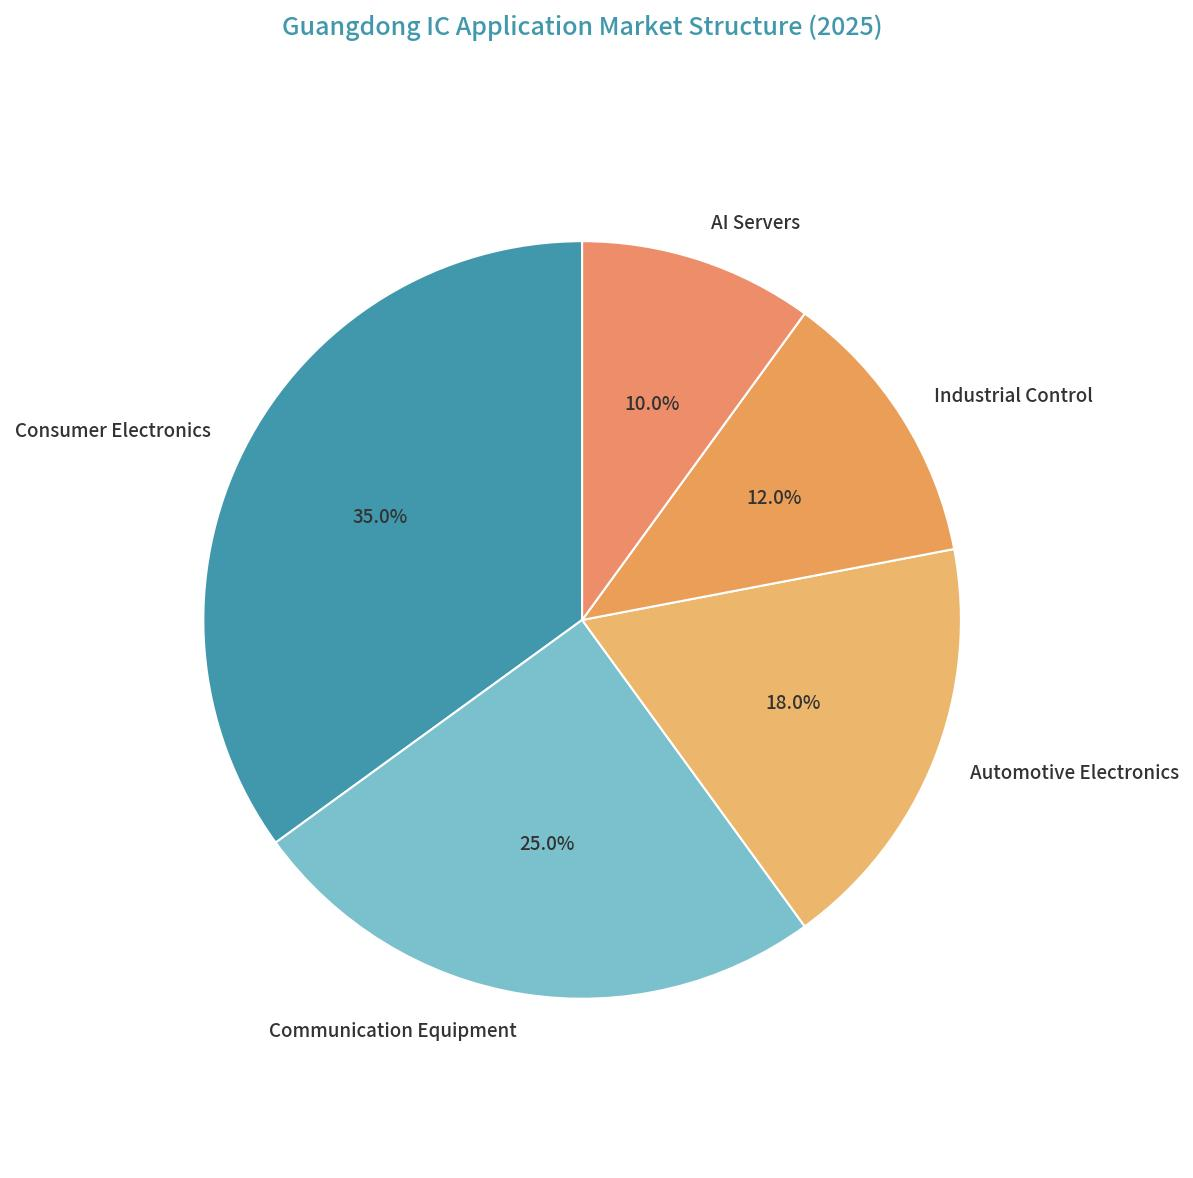
\includegraphics[width=\textwidth]{广东省IC产业应用市场结构.jpeg}
\caption{广东省IC产业下游应用市场结构}
\label{fig:app_market}
\end{figure}

\end{itemize}


\subsection{市场结构与集中度}
\label{sec:market_structure}

\subsubsection{市场集中度（CR5/CR10/CR30）}

基于广东省IC企业名录中企业注册资本计算的
市场集中度分析，揭示了高度寡占的市场结构：

\begin{table}[H]
\centering
\caption{市场集中度指数（基于注册资本）}
\label{tab:concentration}
\begin{tabular}{lrrl}
\toprule
\tableHeaderRow
\textbf{指数} & \textbf{占比 (\%)} & \textbf{累计资本（亿元）} & \textbf{解读} \\
\midrule
\tableOddRow  CR5  & 52.56 & 5,915.55 & 前5名控制超半数行业资本 \\
\tableEvenRow CR10 & 67.15 & 7,556.72 & 前10名控制超三分之二资本 \\
\tableOddRow  CR30 & 88.70 & ---     & 前30名近似垄断资本资源 \\
\bottomrule
\end{tabular}

\vspace{2pt}
{\footnotesize
\textbf{注：}CR指数基于注册资本计算，而非营业收入或市场份额，
仅反映资本集中度特征。}
\end{table}

\textbf{市场结构判断：}CR10达67.15\%，广东IC产业呈现
\textbf{高度寡占型市场结构}，其特征为：
（1）市场支配力高度集中于少数大型企业；
（2）龙头企业在资本规模上拥有绝对竞争优势；
（3）新进入者面临极高的资本壁垒。

这种资本集中与极为分散的企业数量分布（95.3\%为微小型企业）
并存，形成了独特的"资本集中、实体分散"二元结构：少数
资本密集型制造企业掌控了大部分财务资源，
而数千家微设计企业在拥挤的竞争格局中
以极少的资本禀赋谋求生存。
\begin{figure}[H]
\centering
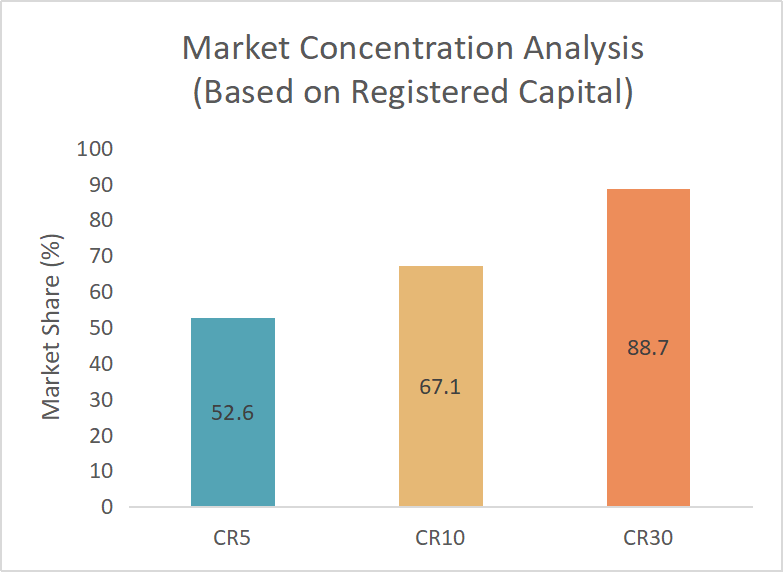
\includegraphics[width=\textwidth]{市场集中度分析.png}
\caption{市场集中度分析（基于注册资本的CR5/CR10/CR30）}
\label{fig:concentration_chart}
\end{figure}


\subsubsection{企业规模结构}

企业规模结构呈现明显的金字塔形态：

\begin{table}[H]
\centering
\caption{不同规模层级的企业类型结构}
\label{tab:enterprise_tiers}
\begin{tabular}{lrrl}
\toprule
\tableHeaderRow
\textbf{层级} & \textbf{数量} & \textbf{占比 (\%)} & \textbf{特征} \\
\midrule
\tableOddRow  中小企业（微型+小型）        & 9,060 & 90.30 & 数量占绝对主导，资本规模极小 \\
\tableEvenRow 规模以上企业                   & 588   & 5.86  & 产业配套骨干力量 \\
\tableOddRow  龙头领先企业                   & 385   & 3.84  & 数量最少，控制主要资本 \\
\bottomrule
\end{tabular}
\end{table}

这种"中小企业为基础、规上企业为骨干、少数龙头企业
为引领"的金字塔结构，表明产业生态基础扎实且具有
较强的创新活力，但产业引领力不足。总体呈现
"大而不强、散而不聚"的特征，整合升级空间广阔。

\subsubsection{所有制结构}

所有制构成揭示了以民营为主导的产业格局：

\begin{itemize}
    \item \textbf{民营企业：}75\%--80\%，是创新和市场开拓的主力军，
          集中在Fabless设计、AI芯片和汽车半导体领域。
    \item \textbf{国有企业：}10\%--15\%，聚焦重资产制造领域，
          包括晶圆制造、存储制造和工业基础设施。
    \item \textbf{外资/合资企业：}5\%--10\%，在高端制造、
          先进封测、EDA软件和半导体设备领域起到补充作用。
\end{itemize}

这种所有制格局反映了更广泛的全国产业格局：
民营企业在AI芯片和RISC-V架构领域主导创新，
国有资本在晶圆制造领域依然关键，外资企业
在先进设备和EDA工具领域保持技术领先。

\subsubsection{区域资本集中度}

资本在空间上的集中度甚至高于企业数量的集中度：

\begin{table}[H]
\centering
\caption{注册资本区域分布（前3城市）}
\label{tab:capital_region}
\begin{tabular}{lrrl}
\toprule
\tableHeaderRow
\textbf{城市} & \textbf{资本额（亿元）} & \textbf{占比 (\%)} & \textbf{角色} \\
\midrule
\tableOddRow  深圳 & 7,866.72 & 69.90 & 核心资本集聚枢纽 \\
\tableEvenRow 珠海 & 2,139.56 & 19.01 & 第二大资本规模城市 \\
\tableOddRow  江门 & 580.02   & 5.15  & 重要资本节点 \\
\bottomrule
\end{tabular}
\end{table}

珠三角九市合计占全省企业数量的95.64\%和注册资本的99.80\%，
呈现出极端的空间集聚特征。非珠三角地区（粤东、粤西、
粤北）在IC资本版图中几乎为零。
\begin{figure}[H]
\centering
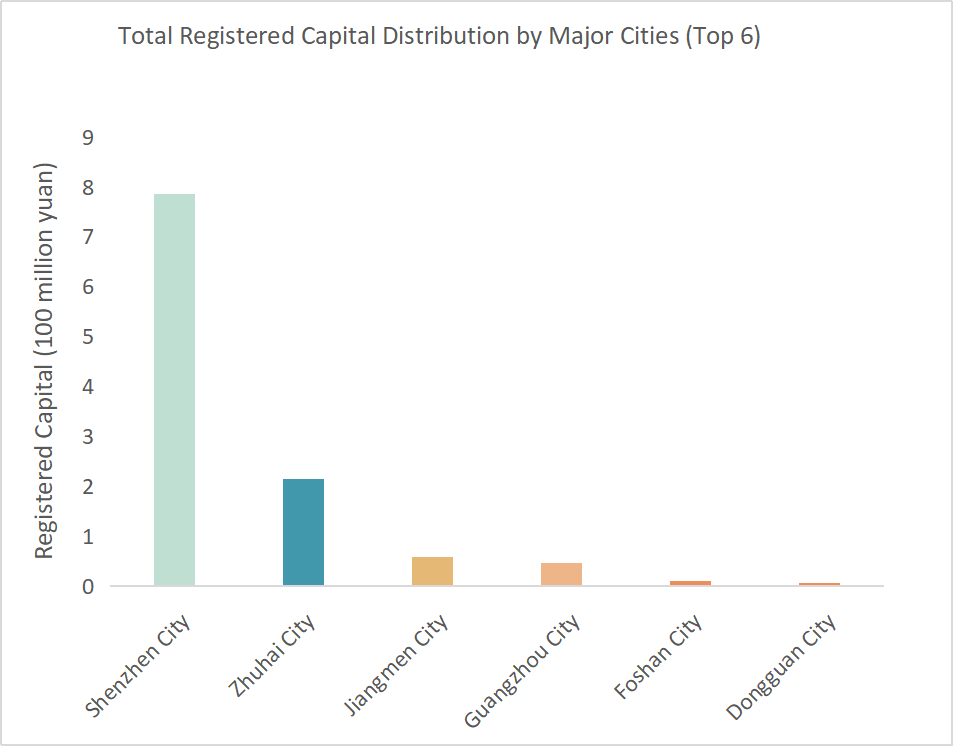
\includegraphics[width=\textwidth]{主要城市总注册资本分布.png}
\caption{主要城市总注册资本分布}
\label{fig:capital_dist}
\end{figure}


% ============================================================
%  第四章 — 人才画像
% ============================================================
\section{人才画像}
\label{sec:talent}

\subsection{人才规模与构成}
\label{sec:talent_scale}

\subsubsection{人才总量与产业分布}

广东省是中国三大集成电路产业核心集群之一。产业布局以IC设计
为核心，以特色工艺制造、先进封测和化合物半导体为延伸，
配套设备与材料企业协同发展。

{\footnotesize\textbf{数据说明：}本节人才数据基于广东省半导体行业协会
对2,000余家重点企业的抽样调查，为估算值而非政府官方统计数据。
数据应视为反映相对规模和结构的指示性数据，而非精确数值。}

全省集成电路全产业链从业人员总数估计约为
\textbf{23.6万人}，约占全国IC从业人员的34\%
（全国约63万人，据《中国集成电路产业人才白皮书（2020--2021）》），
人才集聚度居全国第二位，仅次于长三角。

按产业链环节划分，各环节人才体量与区域产业定位高度匹配：

\begin{table}[H]
\centering
\caption{价值链各环节人才分布}
\label{tab:talent_segment}
\begin{tabular}{p{3.8cm}rrp{6.8cm}}
\toprule
\tableHeaderRow
\textbf{环节} & \textbf{从业人员} & \textbf{占比 (\%)} & \textbf{特征} \\
\midrule
\tableOddRow  IC设计                      & 172,000 & 72.9 & 全国IC设计人才最为集中的区域之一 \\
\tableEvenRow 晶圆制造与特色工艺           & 28,000 & 11.9 & 规模小于长三角；随新晶圆厂建设持续扩张 \\
\tableOddRow  封装测试                    & 24,000 & 10.2 & 集中于珠三角制造城市 \\
\tableEvenRow 设备、材料、EDA与IP支撑     & 12,000 & 5.1 & 支撑人才体系尚处培育阶段 \\
\midrule
\tableOddRow  \textbf{合计} & \textbf{236,000} & \textbf{100.0} & --- \\
\bottomrule
\end{tabular}
\end{table}

\textbf{关键发现：}IC设计是最大的人才板块，占全省IC从业人员近四分之三，
反映了广东作为全国Fabless芯片设计领先者的地位。制造端人才池
相对于长三角仍显不足，制约着全省产能扩张的雄心。
\begin{figure}[H]
\centering
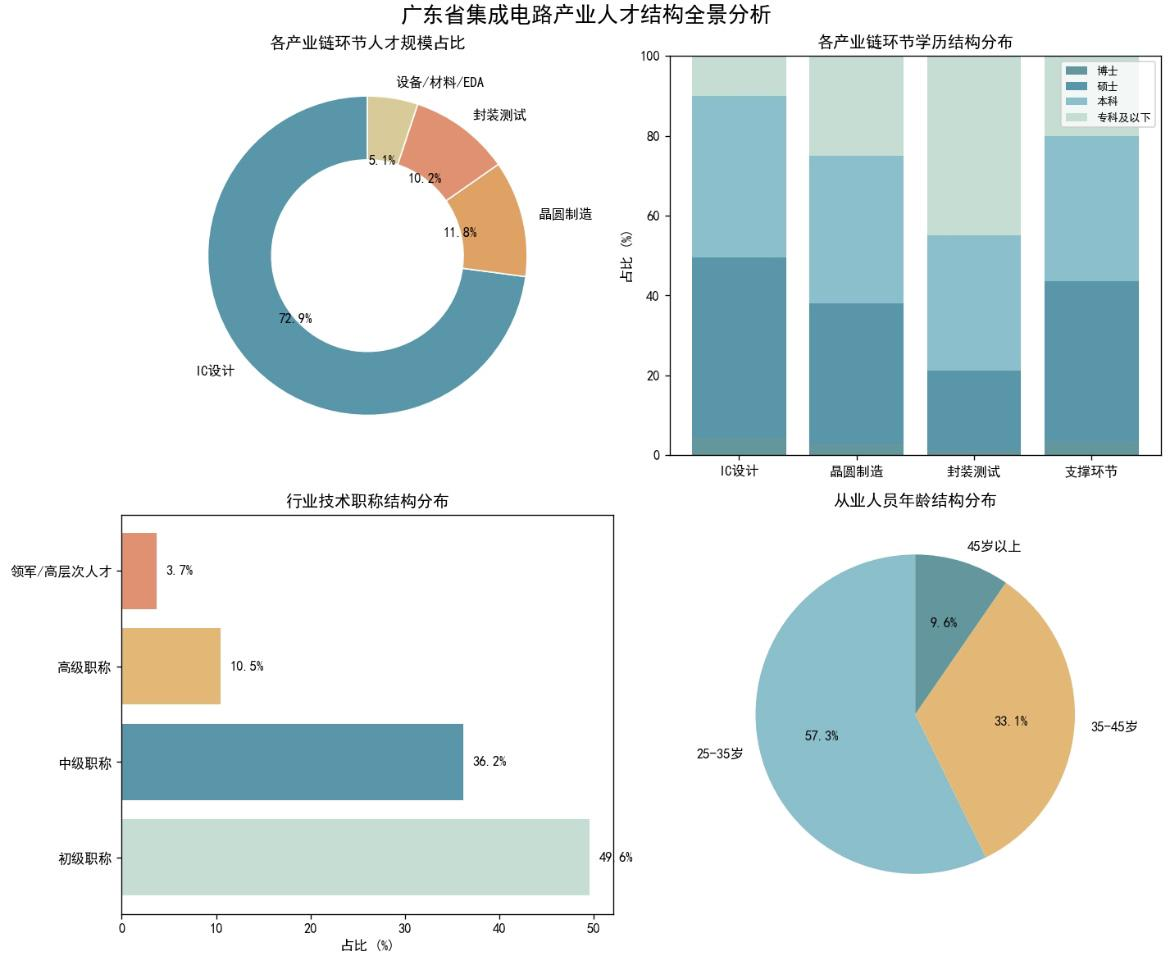
\includegraphics[width=\textwidth]{广东省集成电路产业人才结构全景分析.jpeg}
\caption{广东省集成电路产业人才结构全景分析}
\label{fig:talent_structure}
\end{figure}

全省IC产业当前显性人才缺口约为\textbf{8.7万人}，
其中高端研发、先进工艺、核心IP和EDA工具领域的缺口最大。
随着多条12英寸晶圆产线和第三代半导体产线的持续扩建，
到2027年总人才需求预计将超过\textbf{30万人}，中长期
人才供给压力将持续加大。

\subsubsection{人才区域布局}

广东IC人才呈现高集中度和梯度分布特征，
核心资源集中于珠三角，粤东西北地区几乎为零：

\begin{table}[H]
\centering
\caption{广东省IC人才区域分布}
\label{tab:talent_region}
\begin{tabular}{p{3.5cm}rrp{6.8cm}}
\toprule
\tableHeaderRow
\textbf{城市/区域} & \textbf{从业人员} & \textbf{占比 (\%)} & \textbf{产业聚焦} \\
\midrule
\tableOddRow  深圳              & 138,000 & 58.5 & 设计枢纽：通用芯片、AI芯片、功率IC、射频/模拟 \\
\tableEvenRow 广州              & 32,000 & 13.6 & 制造核心：晶圆代工、特色工艺、研发机构 \\
\tableOddRow  东莞、佛山、中山   & 39,000 & 16.5 & 封测、分立器件、元器件制造 \\
\tableEvenRow 珠海              & 17,000 & 7.2 & 化合物半导体、射频芯片、工控IC设计 \\
\tableOddRow  粤东西北地区       & 少于10,000 & 少于4.2 & 极少：仅有分销和技术服务岗位 \\
\midrule
\tableEvenRow \textbf{合计} & \textbf{236,000} & \textbf{100.0} & --- \\
\bottomrule
\end{tabular}
\end{table}

\textbf{关键发现：}深圳一市即占全省IC从业人员的58.5\%，
前四大城市集群合计占比超过95\%。非珠三角地区在IC人才版图中
几乎为零，研发人才在该区域基本不存在。
\begin{figure}[H]
\centering
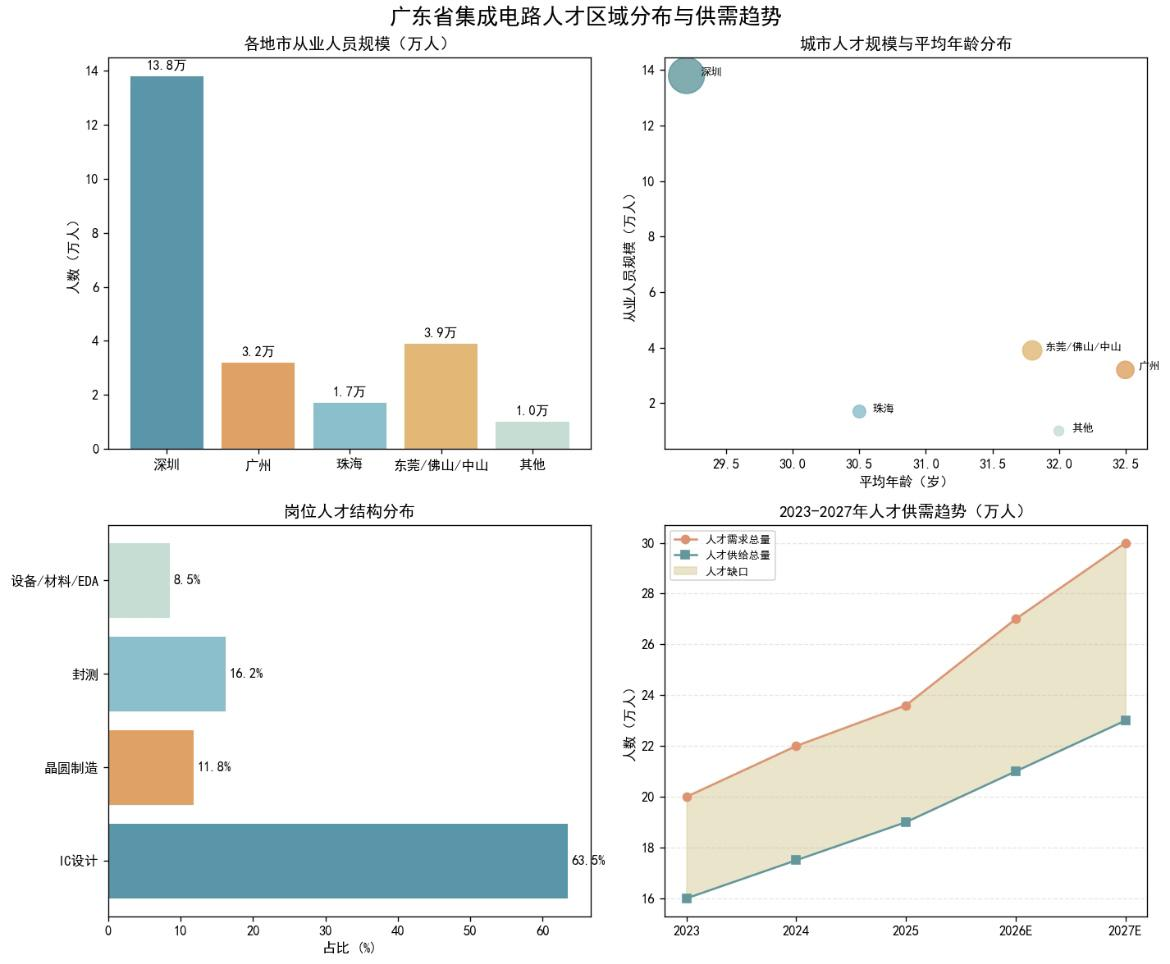
\includegraphics[width=\textwidth]{广东省集成电路人才区域分布与供需趋势.jpeg}
\caption{广东省集成电路人才区域分布与供需趋势}
\label{fig:talent_region_chart}
\end{figure}


\subsubsection{学历背景结构}

据广东省半导体行业协会对2,000余家重点企业的抽样调查，
IC从业人员的学历水平显著高于全省制造业平均水平，
且按价值链环节呈现明显分层：

\begin{table}[H]
\centering
\caption{广东省IC从业人员学历构成}
\label{tab:education}
\begin{tabular}{p{2.6cm}rp{2.5cm}p{7.2cm}}
\toprule
\tableHeaderRow
\textbf{学历层次} & \textbf{占比 (\%)} & \textbf{估计人数} & \textbf{主要岗位} \\
\midrule
\tableOddRow  博士    & 3.3  & 约7,790  & 先进工艺研发、芯片架构、EDA算法、第三代半导体材料 \\
\tableEvenRow 硕士    & 36.8 & 约86,800 & 核心研发：IC设计、工艺研发、芯片验证、后端布局 \\
\tableOddRow  本科    & 37.1 & 约87,500 & 测试、版图设计、工艺执行、设备维护、项目管理 \\
\tableEvenRow 大专及以下 & 22.8 & 约53,900 & 产线操作员、基础品检、现场辅助 \\
\midrule
\tableOddRow  \textbf{本科及以上小计} & \textbf{77.2} & \textbf{约182,000} & --- \\
\bottomrule
\end{tabular}
\end{table}

\textbf{关键发现：}
\begin{itemize}
    \item 77.2\%的从业人员拥有本科及以上学历，远高于
          全省制造业平均水平。
    \item 硕士研究生（36.8\%）是核心研发岗位的主力；
          在深圳和广州的设计企业中，硕士学位
          已成为核心研发岗位的事实上的入职门槛。
    \item 博士层次人才（3.3\%，约7,790人）是最稀缺的群体，
          集中在龙头企业研发中心、高校和科研院所。
    \item 各环节学历分层差异显著：IC设计企业本科以上超90\%，
          晶圆制造约75\%，封测仅约55\%。
\end{itemize}

\subsubsection{职称结构}

IC产业职称结构呈典型金字塔形态，底部庞大、
中部承压、顶部稀缺：

\begin{table}[H]
\centering
\caption{IC从业人员职称结构}
\label{tab:titles}
\begin{tabular}{p{4.5cm}rp{7.5cm}}
\toprule
\tableHeaderRow
\textbf{职称层级} & \textbf{占比 (\%)} & \textbf{特征} \\
\midrule
\tableOddRow  初级（助理工程师、技术员）         & 49.6 & 应届生及3年以下经验者；流动性最强的群体 \\
\tableEvenRow 中级（工程师）                     & 36.2 & 5--10年经验；企业争夺的核心资源 \\
\tableOddRow  高级（高级工程师、教授级）          & 10.5 & 10年以上经验；集中于龙头企业 \\
\tableEvenRow 高层次领军人才与特聘专家            & 3.7 & 行业领军、省级以上高层次人才；全省不足1,000人 \\
\bottomrule
\end{tabular}
\end{table}

\textbf{关键发现：}15年以上工作经验的高级技术人员占比极低，
技术经验和工艺诀窍难以有效传承。全省高层次领军人才总数
不足1,000人，是制约高端产业突破的核心短板。中级工程师
（行业中坚力量）因薪酬和平台竞争面临向长三角的
持续跨区域人才流失。

\subsubsection{年龄结构}

广东IC产业高度年轻化，从业人员平均年龄为
\textbf{30.7岁}，低于全国行业平均水平。但资深技术人才的
结构性断层突出：

\begin{itemize}
    \item \textbf{25--35岁（57.3\%）：}占绝对多数；学习能力强、
          执行力好，但普遍缺乏先进节点（7nm及以下）、
          大规模复杂SoC芯片和车规级高可靠性芯片的全流程项目经验。
    \item \textbf{35--45岁（33.1\%）：}核心技术骨干和基层管理者；
          具有完整的项目经验——但总量不足且面临外部挖角，
          多数企业存在"骨干层不足"的问题。
    \item \textbf{45岁以上（9.6\%）：}资深技术专家和行业老兵，
          具有数十年的积累；人数无法满足先进产线和前沿研发的需求，
          形成了"年轻团队有活力但缺经验、资深人才有经验但
          规模小"的结构性矛盾。
\end{itemize}

在区域差异上，深圳设计企业从业人员平均年龄最低，约29.2岁；
广州制造和科研企业从业人员平均约32.5岁。

\subsection{核心人才需求}
\label{sec:talent_demand}

随着广东从通用型技术人力规模扩张转向攻克
"卡脖子"技术和实现产业自主可控，
人才需求正经历结构性演变——从通用型技术员
转向专精于先进制造、新兴应用和数字化转型的
多学科复合型人才。

\subsubsection{按产业类别的人才需求}

\paragraph{新兴产业：先进制造与研发人才。}
新能源汽车、5G和AI算力的爆发式增长
使研发和制造人才成为最关键的资产：

\begin{itemize}
    \item \textbf{先进工艺人才：}随着技术节点向5nm、3nm及以下推进，
          工艺/良率工程师（PE）需求达到峰值，占IC岗位总需求的
          3.3\%，为需求份额最高的岗位。这些专家对于优化
          量产中的光刻、刻蚀和薄膜工艺至关重要。
    \item \textbf{高端设计人才：}模拟IC设计和数字前端工程师
          是创新的核心驱动力。对于AI芯片，
          需要算法工程师通过量化、剪枝等
          硬件友好方式优化神经网络模型。
\end{itemize}

\paragraph{未来产业：具身智能与先进架构。}
人形机器人和量子计算的前瞻性布局要求
"前瞻性"技能组合：

\begin{itemize}
    \item \textbf{AIoT与具身智能：}工业物联网（IIoT）的发展
          驱动对低功耗、高集成度AIoT芯片的需求。
          工程师必须在硬件算力和软件算法之间取得平衡，
          实现"大脑"与"身体"的协同。
    \item \textbf{Chiplet与先进架构：}随着摩尔定律放缓，
          Chiplet和存内计算技术正在革新芯片设计。
          架构师必须具备超越传统冯·诺依曼瓶颈的能力，
          以服务数据中心和AI工作负载。
\end{itemize}

\paragraph{传统产业：数字化转型与功率半导体。}
传统制造业的数字化转型催生嵌入式系统
和第三代半导体应用需求：

\begin{itemize}
    \item \textbf{数字化转型专才：}嵌入式软件开发和驱动开发
          需求保持稳定（约占岗位的2.1\%），这些专业人才
          将IC技术融入传统设备，实现互联互通和
          智能化。
    \item \textbf{第三代半导体：}碳化硅（SiC）和氮化镓（GaN）
          在新能源汽车和快充领域的渗透
          需要具备高耐热、低损耗材料经验的材料研发工程师。
\end{itemize}

\subsubsection{价值链各环节需求}

各价值链环节关键紧缺岗位汇总如下：

\begin{table}[H]
\centering
\caption{价值链各环节核心人才缺口}
\label{tab:talent_shortage}
\begin{tabular}{p{2.5cm}p{7cm}p{3.5cm}}
\toprule
\tableHeaderRow
\textbf{环节} & \textbf{关键紧缺岗位} & \textbf{紧缺程度} \\
\midrule
\tableOddRow  IC设计 & 模拟IC设计、数字前端/后端、EDA软件开发、AI芯片算法工程师 & 紧缺强度最高 \\
\tableEvenRow 晶圆制造 & 工艺研发工程师、光刻/刻蚀/薄膜/离子注入工程师、良率提升工程师、产线整合工程师 & 缺口快速扩大 \\
\tableOddRow  封装测试 & 先进封装研发（SiP/FC/WLCSP）、Fan-out/2.5D/3D封装工程师 & 新兴方向，储备不足 \\
\tableEvenRow 设备与材料 & 半导体设备研发、关键材料研发（光刻胶、特种气体、溅射靶材）、EDA工具研发 & 最薄弱环节；全省全职EDA/IP专业人员不足4,500人 \\
\bottomrule
\end{tabular}
\end{table}

\subsubsection{岗位结构与供需特征}

结合产业链形态，岗位结构具有鲜明的区域特征：

\begin{itemize}
    \item \textbf{IC设计岗位（占总岗位的63.5\%）：}数字IC设计和
          芯片验证需求最强；模拟/射频IC设计和电源管理芯片设计
          为传统优势岗位，人才门槛高、培养周期长，面临
          持续性长期缺口。AI芯片和车规级芯片设计
          人才需求为近三年增长最快。
    \item \textbf{晶圆制造与工艺岗位（11.8\%）：}随着多条特色工艺
          和第三代半导体产线的落地，工艺工程师缺口持续扩大。
          广东制造人才池起步较晚，成熟工艺工程师
          高度依赖外部引进。
    \item \textbf{封装测试岗位（16.2\%）：}传统封装人才供给较为充足；
          Fan-out、2.5D/3D先进封装为新兴方向，技术储备不足。
    \item \textbf{设备、材料、EDA与IP支撑（8.5\%）：}最薄弱环节——
          全省全职EDA研发与IP开发专业人员不足4,500人；
          核心工具和自主IP领域几乎完全依赖外部人才引进和采购。
\end{itemize}

\subsubsection{核心技能与资格要求}

据行业调研，企业当前更强调"硬科技"与"软技能"的平衡：

\begin{itemize}
    \item \textbf{专业知识：}扎实的电子工程、微电子、物理和
          数学基础；熟练使用EDA工具（Cadence、Synopsys）为必备条件。
    \item \textbf{技术深度：}射频工程师需精通高频
          与小型化设计；验证工程师需熟练掌握
          UVM架构和FPGA原型验证。
    \item \textbf{跨学科能力：}随着SoC复杂度提升，
          横跨电子、计算机科学和软件知识的
          "T型"人才备受青睐。
    \item \textbf{协作能力：}跨"设计--制造--测试"
          链有效沟通的能力，对确保设计
          准确性和快速良率爬坡至关重要。
\end{itemize}

\subsubsection{经验偏好与招聘特征}

招聘模式呈现明显的"实干导向"偏好：

\begin{itemize}
    \item \textbf{项目经验优先：}企业强烈偏好具有可证明的项目履历、
          能立即解决良率提升或失效分析等现场问题的工程师。
          应届生通常需要3--12个月的二次培训后方能独立上岗。
    \item \textbf{中型企业最活跃：}100--499人规模的企业
          是主要招聘方（占岗位发布的25.7\%），
          反映其快速扩张阶段对"即插即用"
          型人才的迫切需求。
    \item \textbf{跨行业人才流入：}IC产业虽以行业内人才流动为主，
          但随着技术技能日益可转移，来自机械/设备（4.96\%）、
          互联网（4.17\%）和计算机软件（4.05\%）行业的
          流入显著。
\end{itemize}

\subsection{人才分布与流动}
\label{sec:talent_flow}

\subsubsection{空间集中度与全国格局}

中国IC人才高度集中于三大城市群：长三角（上海+无锡+南京+苏州+杭州+合肥，
约40万人）、珠三角（广东省约23.6万人）和京津冀（北京+天津，
约14万人）。三大区域合计占全国IC从业人员（全国约63万人）
的85\%以上。

在这一全国版图中，上海（约20万人）、深圳（约13.8万人）、
北京（约13万人）构成第一梯队，合计约占全国总量的48\%。
\begin{figure}[H]
\centering
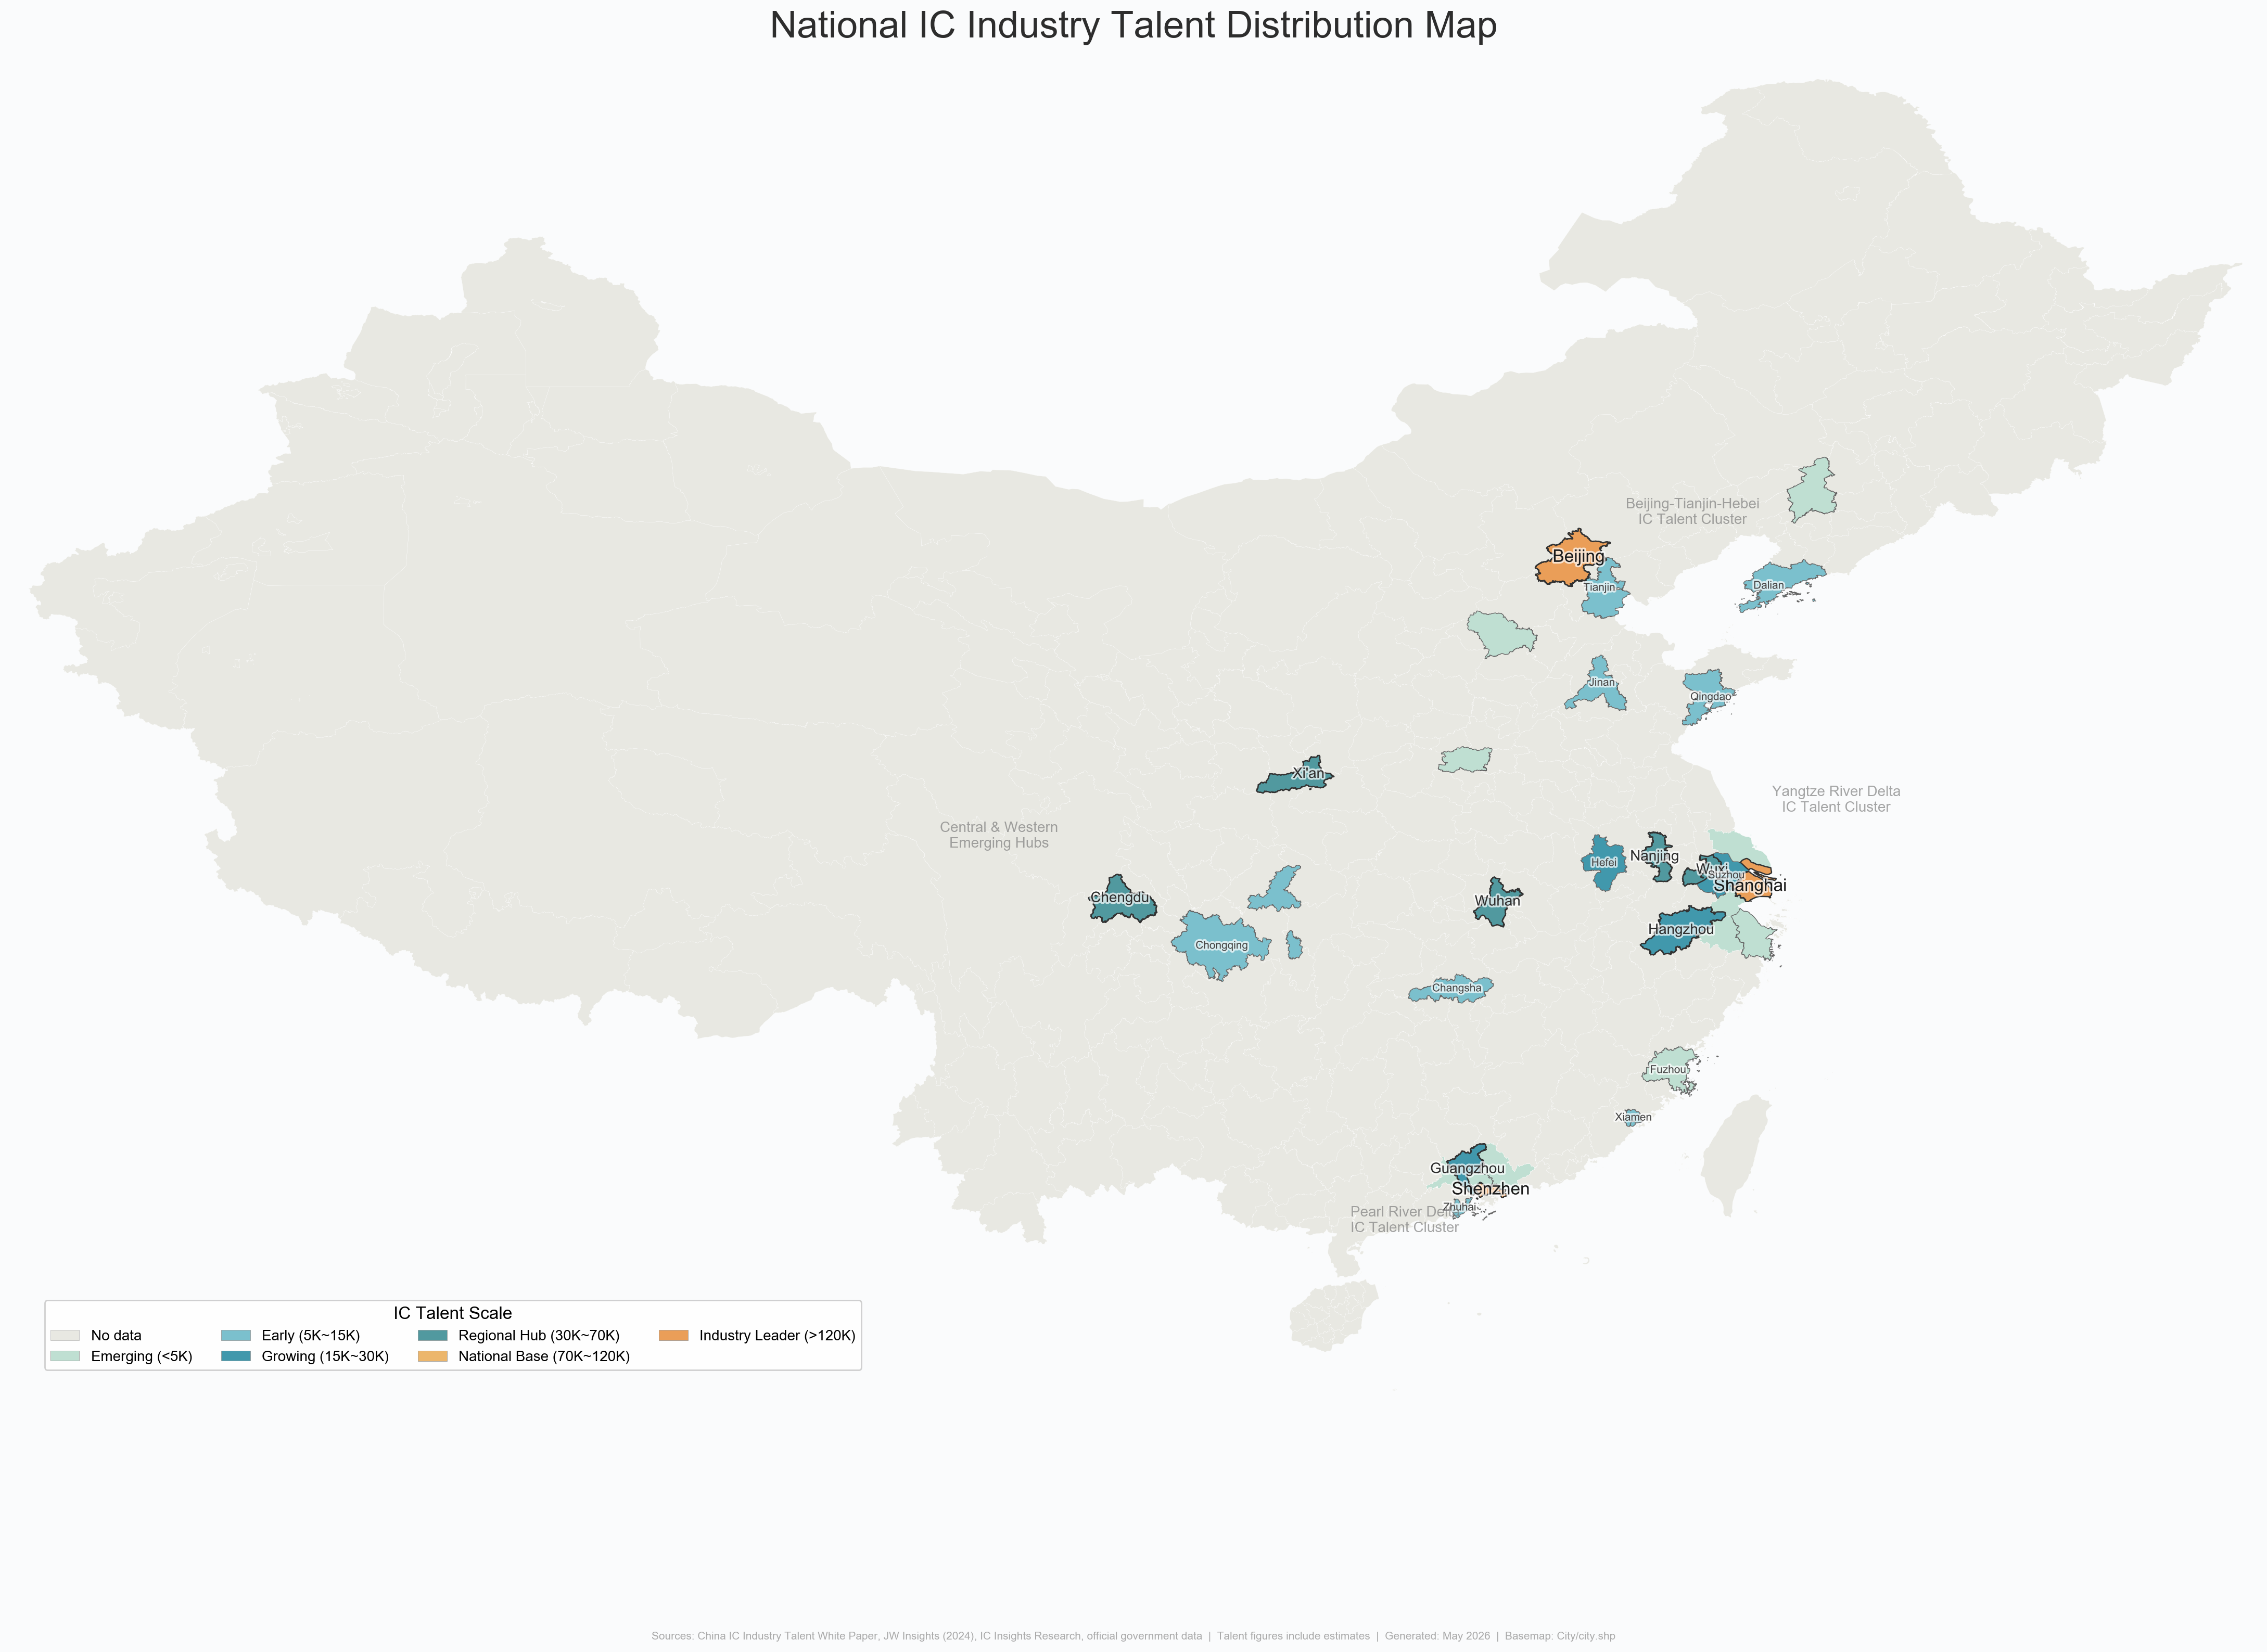
\includegraphics[width=\textwidth]{全国IC人才分布图_en.png}
\caption{全国集成电路产业人才分布图}
\label{fig:talent_map}
\end{figure}

\subsubsection{省内流动格局}

商业人力资源平台数据（猎聘，2024年）记录了珠三角核心城市间的
人才双向流动：

\begin{table}[H]
\centering
\caption{各城市人才输送来源构成（猎聘2024）}
\label{tab:talent_flow_cities}
\begin{tabular}{p{3.5cm}p{9.5cm}}
\toprule
\tableHeaderRow
\textbf{输送目的地} & \textbf{主要来源地（占总输送量\%）} \\
\midrule
\tableOddRow  广州 & 本地 42.13\%, 深圳 8.17\%, 佛山 3.76\%, 东莞 2.87\% \\
\tableEvenRow 深圳 & 本地 37.58\%, 广州 7.45\%, 上海 4.63\%, 北京 3.86\% \\
\tableOddRow  东莞 & 本地 27.46\%, 深圳 16.12\%, 广州 8.91\% \\
\bottomrule
\end{tabular}

\vspace{2pt}
{\footnotesize
\textbf{注：}猎聘平台数据反映自愿求职行为，
不等同于官方政府统计数据；此处仅作为
人才流动模式的方向性指示使用。}
\end{table}

\textbf{关键发现：}
\begin{itemize}
    \item 深圳表现出较强的人才留存能力（37.58\%本地），但也
          存在向广州、上海、北京的显著流出，受
          薪酬、平台和生活成本的竞争驱动。
    \item 东莞本地留存率最低（27.46\%）而对深圳的依赖度最高
          （16.12\%），反映其作为制造业腹地
          承接深圳溢出的角色。
    \item 对IC行业的跨行业流入主要源自
          电子/半导体/IC行业本身（7.86\%），其次为
          机械/设备（4.96\%）、互联网（4.17\%）和
          计算机软件（4.05\%）。
\end{itemize}

\subsubsection{政府引才举措}

2026年，广东省启动"百万英才汇南粤"N城联动招聘
活动，覆盖北京、上海、南京、杭州等主要IC产业
集聚城市。仅深圳一市即携120余家省内重点企业
和1万余高质量岗位，赴北京大学、
清华大学、复旦大学和上海交通大学等8所顶尖高校。
招聘聚焦IC、AI、生物医药和低空经济等战略性
新兴产业——其中年薪50万--100万的岗位超2,000个，
年薪超100万的岗位超120个。

深圳市采取"引育留"多措并举的方式
构建多层次IC人才队伍：完善人才引进机制
招募全球行业领军人才；推动南科大和深圳大学
等10所高校开设IC相关专业；借助较低的落户门槛
和创新产业环境，连续多年位居全国最吸引
95后人才城市前列。

\subsubsection{高校人才培养与留存}

\paragraph{招生规模扩大。}广东省IC相关专业点数量
已从2022年的7个扩展至32个，总招生规模
（本科至博士）超1万人——较2022年增长4倍。
深圳大学IC工程硕士专业近五年就业率保持100\%，
其中94.3\%签约就业于华为海思、中兴微、ADI、百度等企业。

\paragraph{六大省级IC人才培养基地。}2022年12月，广东省
教育厅正式批准六所高校——华南理工大学（SCUT）、中山大学（SYSU）、
南方科技大学（SUSTech）、深圳大学（SZU）、广东工业大学（GDUT）和
珠海科技学院（ZCST）——设立"广东省集成电路人才培养基地"。

\paragraph{四种产学研合作模式。}

\begin{table}[H]
\centering
\caption{IC人才培养产学研合作模式}
\label{tab:u-i_models}
\begin{tabular}{p{2.8cm}p{5.6cm}p{5.2cm}}
\toprule
\tableHeaderRow
\textbf{模式} & \textbf{典型案例} & \textbf{合作企业/机构} \\
\midrule
\tableOddRow  定制培养班 & 广工--粤芯"匠心班"；广工与30余家企业定制班 & 粤芯半导体、华为、全志科技 \\
\tableEvenRow 联合实验室 & 南科大深港微电子联合实验室；深大--华为EDA联合实验室；广工--华为"鲲鹏\&昇腾"开发者创新俱乐部（全国首家） & 华为、中兴微、安谋中国、中芯国际、紫光展锐 \\
\tableOddRow  产业学院   & 广工集成电路学院（2021年10月成立）；深圳技术大学计算微电子学院 & 华为、粤芯半导体、五个工信部电子所 \\
\tableEvenRow 联合培养研究生 & 省集成电路行业协会联合培养基地；工程硕博士改革专项 & 佛山、东莞、中山、汕头+省农科院；已培养超6,000名研究生 \\
\bottomrule
\end{tabular}
\end{table}

\subsubsection{核心结构性问题}

尽管进展迅速，广东IC人才格局仍存在五大核心结构性问题：

\begin{enumerate}[label=(\arabic*)]
    \item \textbf{高端核心人才严重短缺：}芯片架构师、
          先进工艺工程师、EDA研发专家和车规级芯片
          安全认证专家缺口超过70\%。本地培养速度
          远落后于产业扩张速度，严重依赖外部引进。
    \item \textbf{骨干人才稳定性不足：}35岁左右的成熟工程师——
          产业最迫切需求的群体——因薪酬、平台和
          生活成本等因素在城市和区域间频繁流动，
          企业难以回收培养投入。
    \item \textbf{产教融合不够深入：}开设IC相关专业的
          高校和职业院校数量仍有限，课程设置与
          实际岗位需求脱节。应届生通常需3--12个月
          二次培训，无法实现"毕业即上岗"。
    \item \textbf{长期人才梯队断层：}15年以上工作经验的
          高级技术人员占比极低，技术经验和工艺诀窍
          难以跨代有效传承。
    \item \textbf{价值链人才发展不均衡：}设计环节人才拥挤且竞争激烈，
          而重资产、长周期环节（制造、设备、材料）
          人才吸引力不足，制约全链条协同发展。
\end{enumerate}

\subsection{人才政策对接}
\label{sec:talent_policy}

\subsubsection{多层次政策体系概览}

省、市、区各级政府对集成电路人才推出了
多方位政策包。但在全产业链维度上，
现有政策在覆盖面上呈现出明显的结构性不均衡。

\paragraph{省级层面：战略性引才与宏观激励。}
广东省通过广东优粤卡、粤港澳大湾区个人所得税优惠
（对境外高端和紧缺人才给予个税差额补贴，将实际税负
上限控制在15\%）、高等教育"冲补强"提升计划
和基础学科人才培养项目等多项举措，
扩大本地人才池。广东集成电路人才培养数量
在"十四五"期间翻了两番。

\paragraph{市区级层面。}
深圳、广州、珠海各市均推出了针对性人才激励措施，包括深圳的研发团队最高500万元奖励、
广州南沙每人每年最高300万元的个税返还、珠海横琴的MPW流片专项综合补贴等。
详细政策内容见第~\ref{sec:municipal_policy}~节。

\subsubsection{各类人才的政策覆盖与适配性}

现有人才政策对不同岗位、不同学历背景的从业者
呈现出不均匀的覆盖面和适配度。
{\footnotesize 以下覆盖率为课题组根据政策文件分析综合得出的
示意性估计值，不代表官方统计数据，旨在说明各类人才
政策关注度的相对差异。}

\begin{table}[H]
\centering
\caption{IC各类人才政策覆盖率（课题组估计）}
\label{tab:policy_coverage}
\begin{tabular}{p{3.5cm}rp{7.5cm}}
\toprule
\tableHeaderRow
\textbf{人才类别} & \textbf{估计覆盖率 (\%)} & \textbf{评估} \\
\midrule
\tableOddRow  IC设计人才    & 约95 & 地方政策核心聚焦；研发奖励、个税补贴、流片激励均向设计端倾斜 \\
\tableEvenRow 制造与封测工程人才 & 约80 & 随新一轮制造发力逐步覆盖，但传统评价门槛（纳税、学历）可能排斥制造工程师 \\
\tableOddRow  应用与测试技术人才   & 约60 & 专项补贴少；多纳入通用青年人才或企业评价名额 \\
\tableEvenRow 一线技能人才          & 约35 & 覆盖率最低；仅限于落户和公租房支持；对晶圆厂操作人员的定向激励不足 \\
\bottomrule
\end{tabular}
\end{table}

\textbf{关键发现：}设计环节人才享受近乎全面的政策覆盖（约95\%），
受益于研发团队奖励、个税补贴和流片激励。相比之下，
一线技能人才——对晶圆制造和封测运营至关重要——
仅获约35\%的覆盖率，导致制造环节持续存在
长期用工短缺。

\subsubsection{人才薪酬水平}

广东IC产业薪酬水平居全国前列。
深圳IC设计薪酬与上海、北京基本持平，
形成全国IC人才薪资最高的三大区域：

\begin{itemize}
    \item \textbf{高壁垒岗位（爆发式增长）：}对攻克技术瓶颈至关重要的
          核心岗位——数字前端设计、模拟芯片设计和算法开发——
          月薪中位约3.5万元，年终奖普遍高于行业平均水平。
          8年以上经验的资深人才年薪可达
          80万--120万+。
    \item \textbf{制造环节（稳定增长）：}晶圆代工厂的工艺工程师
          和设备工程师薪资增长较为温和。应届本科生
          月薪1万--1.5万元；1--3年经验者
          月薪1.5万--2.2万元。制造业的薪资增长率
          显著低于前端设计。
    \item \textbf{核心管理岗位：}一线城市（深圳、广州）IC产品线
          总经理、副总经理年薪中位超95万元，
          90分位值超120万元——较二线城市
          高出约20\%。
\end{itemize}

\subsubsection{产业竞争力评价}

将广东省IC人才环境与长三角（上海、无锡、苏州）
及中西部（成都、西安、武汉）进行横向比较，
得出如下SWOT评估：

\begin{table}[H]
\centering
\caption{广东省IC人才竞争力SWOT矩阵}
\label{tab:talent_swot}
\begin{tabular}{p{7cm}p{7cm}}
\toprule
\tableHeaderRow
\textbf{优势（Strengths）} & \textbf{劣势（Weaknesses）} \\
\midrule
\tableOddRow
$\bullet$ 全国最大的终端应用市场（消费电子、新能源汽车、AI） &
$\bullet$ 晶圆制造和EDA领域的龙头基础企业相对于长三角仍发育不足 \\
$\bullet$ 粤港澳大湾区一体化下独特的15\%境外人才个税优惠 &
$\bullet$ 深圳、广州极高的居住和生活成本制约人才留存 \\
$\bullet$ 毗邻港澳的跨境人才吸引优势 &
$\bullet$ IC制造生态系统仍处于早期培育阶段 \\
\midrule
\tableHeaderRow
\textbf{机遇（Opportunities）} & \textbf{威胁（Threats）} \\
\midrule
\tableOddRow
$\bullet$ 高校战略性扩招（5年增长4倍）加速本地人才供给管道 &
$\bullet$ 长三角成熟生态系统的强大引力，无锡、苏州更具成本优势 \\
$\bullet$ "粤港澳大湾区博士后"创新平台与"揭榜挂帅"机制加速科研成果转化 &
$\bullet$ 中西部城市（成都、西安、武汉）以更低生活成本分流制造人才 \\
\bottomrule
\end{tabular}
\end{table}

\textbf{核心竞争挑战：}高生活成本造成持续性人才留存困境。
年薪30万--50万的3--5年经验的中层工程师，
极易被无锡、苏州、成都和西安等
具有扎实产业基础和更可负担住房的替代城市吸引。
广东能够以有竞争力的薪酬招到人才，却难以持续留住他们。这种
"旋转门"效应，叠加长三角在制造人才积累方面十多年的
先发优势，构成了广东IC人才战略最
重大的结构性挑战。

% ============================================================
%  第五章 — 集群竞争力分析
% ============================================================
\section{集群竞争力分析}
\label{sec:cluster}

\subsection{理论基础}
\label{sec:theory}

产业集群竞争力并非自发形成的结果，而是要素禀赋、市场动态、制度环境和空间组织之间系统互动的产物。本报告采用两个互补的理论框架——迈克尔·波特的\textbf{钻石模型}（1990年）和大卫·李嘉图的\textbf{比较优势理论}（1817年，经赫克歇尔--俄林及后续学者扩展）——来构建广东IC集群竞争力的分析。

\subsubsection{波特的钻石模型}

波特（1990年）认为，国家——进而区域——的竞争优势是创造出来的而非继承而来的，它存在于一个地区在特定产业中配置资源的生产力之中。钻石模型识别出六个相互依存的决定因素：

\begin{enumerate}[label=(\arabic*)]
    \item \textbf{生产要素条件。}涵盖一个地区的生产要素禀赋：人力资源、物质资源、知识资源、资本资源和基础设施。波特区分了\textit{初级要素}（自然禀赋、非熟练劳动力）和\textit{高级要素}（专业人才、研发能力），高级要素是可持续竞争优势的真正驱动力。
    \item \textbf{需求条件。}本地需求的性质和成熟度塑造创新的步伐和方向。广东受益于中国最大的IC应用市场。
    \item \textbf{相关与支持性产业。}具有国际竞争力的供应商和相关产业的存在会强化一个产业的竞争优势——包括EDA软件、半导体设备、特种化学品、硅晶圆和测试服务。
    \item \textbf{企业战略、结构与竞争。}活跃的国内竞争驱动企业升级和创新。广东的IC版图包含大型平台（华为海思、中兴微）、上市Fabless公司以及大量中小微设计企业。
    \item \textbf{政府。}政府通过补贴、税收政策、教育投资和监管框架塑造商业环境。在中国半导体产业中，政府扮演着尤为突出的角色。
    \item \textbf{机遇。}随机事件——技术突破、供应链转移——可以重塑竞争地位。2019年以来的中美科技脱钩构成了一次重大机遇事件。
\end{enumerate}

\subsubsection{比较优势理论}

比较优势理论回答了一个区域\textit{应该将资源投向何处}的问题。应用于IC产业：IC设计是人力资本密集型的；晶圆制造是资本密集型的；封装测试相对劳动密集型；设备/材料则需要深厚的科技联动。广东的比较优势在于设计人才和电子供应链，而制造和设备环节需要通过有意投资高级要素来向高附加值环节转移。

\subsection{广东三大核心IC集群概览}
\label{sec:cluster_overview}

集成电路产业是信息技术产业的核心组成部分，也是广东省重点培育的战略性新兴产业之一。经过多年发展，广东已形成以深圳、广州、珠海为核心的三大IC产业集群。深圳聚焦芯片设计与技术创新，广州主攻晶圆制造，珠海则在第三代半导体领域形成了竞争优势。三市共同构成了广东IC产业的主要增长引擎，并与东莞、佛山、中山等城市形成了"3+N"的空间格局，在封装测试和终端应用环节提供支撑。

\begin{table}[H]
\centering
\small
\caption{广东省三大IC产业集群综合对比}
\label{tab:three_clusters}
\begin{tabular}{p{2.5cm}p{3.5cm}p{3.5cm}p{3.5cm}}
\toprule
\tableHeaderRow
\textbf{维度} & \textbf{深圳集群} & \textbf{广州集群} & \textbf{珠海集群} \\
\midrule
\tableOddRow 产业定位 & 芯片设计与创新中心 & 晶圆制造中心 & 第三代半导体基地 \\
\tableEvenRow 代表企业 & 海思、中兴微、汇顶科技 & 粤芯半导体、上海先进半导体 & 英诺赛科、全志科技、杰理科技 \\
\tableOddRow 企业数量（2024） & 727家 & 约200家 & 100余家 \\
\tableEvenRow 产业规模 & 2839.6亿元 & 约500亿元 & 约200亿元 \\
\tableOddRow 主要专利领域 & AI芯片、EDA、通信芯片 & 制造工艺、车规芯片 & GaN功率器件 \\
\tableEvenRow 技术突破 & 国产IP核、EDA工具、车规芯片 & 12英寸特色工艺量产 & GaN快充芯片商业化 \\
\tableOddRow 政策重点 & 研发支持与流片补贴 & 制造扩产与设备补贴 & 第三代半导体专项支持 \\
\tableEvenRow 区位优势 & 强大的电子产业生态 & 汽车产业与高校资源 & 消费电子供应链完整、成本较低 \\
\tableOddRow 供应链角色 & 芯片设计 & 晶圆制造 & 功率与特色半导体 \\
\bottomrule
\end{tabular}
\end{table}

\subsection{深圳集群：设计与创新中心}
\label{sec:sz_cluster}

深圳在广东IC集群中拥有最强的创新能力。截至2024年底，深圳共有727家IC企业，其中设计企业456家，占比62.7\%。产业实现营收2839.6亿元，同比增长32.9\%，约占广东IC产业总产出的79\%。深圳在人工智能芯片、通信芯片、车规级芯片和EDA软件等领域形成了强大的创新能力。全省超过65\%的IC相关发明专利集中在深圳，凸显了其作为主要创新引擎的地位。

深圳受益于华为、腾讯、比亚迪、大疆等领先科技企业的集聚效应。其强大的电子制造生态创造了"市场需求驱动芯片创新"的发展模式。风险投资机构和高科技人才的集中也为深圳提供了显著的创新优势。重点企业包括海思（位居全球Fabless前十）、中兴微电子（通信芯片）、中芯国际深圳（先进代工）和深南电路（高端PCB基板）。

\subsection{广州集群：晶圆制造中心}
\label{sec:gz_cluster}

广州在制造创新中扮演关键角色，着力弥补广东在晶圆制造领域的历史短板。依托粤芯半导体12英寸特色工艺生产线——粤港澳大湾区首条实现量产的12英寸晶圆代工线——该市聚焦模拟芯片、功率器件和车规级半导体制造技术的突破。2024年，广州IC产出同比增长68.9\%。

集群发展的关键驱动力是龙头企业（"链主"）的垂直整合能力。粤芯半导体已启动四期项目，其第四期投资252亿元，旨在从纯模拟代工平台转型为"模拟为核、数字升级、光电融合"的混合技术平台。以粤芯为锚点，广州开发区已集聚超150家IC企业，形成了"设计--制造--封测--设备/材料--终端应用"的完整生态。

黄埔区实现了精细化的空间分工：知识城（北部）承载制造、科学城（中部）承载设计创新、港区（南部）承载终端应用，加速了从研发到商业部署的协调效率。广州地处珠三角地理中心，拥有广汽集团等汽车产业资源和华南理工大学、中山大学等高校资源，进一步增强了集群竞争力。

\subsection{珠海集群：第三代半导体基地}
\label{sec:zh_cluster}

珠海通过英诺赛科、全志科技和杰理科技等企业崛起为第三代半导体重要中心。英诺赛科建立了国内领先的氮化镓（GaN）产业化平台，实现了8英寸GaN-on-Si量产，使珠海成为国家第三代半导体发展的重要枢纽。全志科技和杰理科技分别在智能音视频SoC和蓝牙芯片领域占据领先地位。

珠海紧邻中山、佛山等制造中心，拥有完善的消费电子和电源产业生态。较低的土地和运营成本使其对半导体制造和规模化生产项目尤其具有吸引力。该市设立了1亿元产业基金支持细分设计企业，设计环节近年的年均增长率超过20\%。

\subsection{技术创新能力对比}
\label{sec:innovation_compare}

技术创新是产业集群竞争力的关键决定因素。广东已形成以深圳为创新枢纽、广州为制造创新基地、珠海为第三代半导体专业中心的创新体系。

\begin{table}[H]
\centering
\caption{专利与创新能力对比}
\label{tab:innovation_compare}
\begin{tabular}{p{2.5cm}p{3.5cm}p{3.5cm}p{3.5cm}}
\toprule
\tableHeaderRow
\textbf{指标} & \textbf{深圳} & \textbf{广州} & \textbf{珠海} \\
\midrule
\tableOddRow 创新主体 & IC设计企业 & 制造企业 & 功率半导体企业 \\
\tableEvenRow 占全省发明专利比重 & $>$65\% & 约20\% & 约10\% \\
\tableOddRow 主要专利领域 & AI芯片、EDA、通信芯片 & 制造工艺、车规芯片 & GaN功率器件 \\
\tableEvenRow 创新特征 & 原创创新强 & 工艺创新强 & 产业化能力强 \\
\tableOddRow 全国竞争力 & 第一梯队集群 & 专业制造基地 & 第三代半导体领先基地 \\
\bottomrule
\end{tabular}
\end{table}

从专利分布和技术突破来看，深圳集中了广东大部分高价值发明专利，是全省的创新中心。广州聚焦制造工艺创新，珠海专攻第三代半导体创新。三市共同形成了差异化创新生态，提升了广东整体产业竞争力。

\subsection{产业链协作分析}
\label{sec:chain_collaboration}

广东已建立起相对完整的集成电路产业链。2024年，全省IC产业总产出约3600亿元，其中芯片设计2109亿元（58.6\%）、封装测试795亿元（22.1\%）、晶圆制造92亿元（2.6\%）、设备与材料608亿元（16.9\%）。

\begin{table}[H]
\centering
\caption{广东省IC产业链分工格局}
\label{tab:chain_division}
\begin{tabular}{p{3cm}p{4cm}p{6cm}}
\toprule
\tableHeaderRow
\textbf{产业链环节} & \textbf{主要城市} & \textbf{代表企业} \\
\midrule
\tableOddRow 芯片设计 & 深圳 & 海思、汇顶科技、中兴微电子 \\
\tableEvenRow 晶圆制造 & 广州 & 粤芯半导体 \\
\tableOddRow 功率半导体 & 珠海 & 英诺赛科 \\
\tableEvenRow 封装测试 & 东莞、佛山、中山 & 天域半导体等 \\
\tableOddRow 终端应用 & 深圳、东莞 & 华为、比亚迪、大疆 \\
\bottomrule
\end{tabular}
\end{table}

\begin{table}[H]
\centering
\caption{产业链完整性评估}
\label{tab:chain_completeness}
\begin{tabular}{p{4.5cm}p{8.5cm}}
\toprule
\tableHeaderRow
\textbf{环节} & \textbf{发展状况} \\
\midrule
\tableOddRow 芯片设计 & 竞争优势强 \\
\tableEvenRow 晶圆制造 & 快速提升中 \\
\tableOddRow 封装测试 & 较为成熟 \\
\tableEvenRow 设备与材料 & 相对薄弱 \\
\tableOddRow EDA软件 & 有待进一步发展 \\
\bottomrule
\end{tabular}
\end{table}

区域协作模式——"设计（深圳）--制造（广州）--封测（东莞、佛山、中山）--应用（深圳、东莞）"——有助于降低供应链成本、提升资源配置效率、增强广东整体产业竞争力。这种"市场拉动+制造追赶+链主带动"的模式正加速广东成为中国IC第三极的进程。

尽管广东已建立较为完整的IC产业链，但在先进半导体设备、光刻技术和EDA软件等关键领域仍面临挑战。未来发展应聚焦于实现这些关键技术的突破，深化"设计--制造--应用"闭环协同，并推进硅光子和先进封装能力建设。

\subsection{省级集群钻石模型分析}
\label{sec:provincial_cluster}

本节运用波特的钻石模型，对广东IC集群的六个决定因素进行系统评估。

\subsubsection{生产要素条件}

广东IC生产要素条件详见第二至四章，从钻石模型视角可概括如下。
\textbf{人力资源}（见第~\ref{sec:talent_scale}~节）：约23.6万从业人员集中于深圳和广州，
人才结构以设计为主（72.9\%），77.2\%拥有本科及以上学历。
\textbf{物质与知识资源}（见第~\ref{sec:enterprises}~节和第~\ref{sec:infrastructure}~节）：
94.1\%的企业集中在珠三角；IC布图设计登记量全国领先；关键平台包括粤芯半导体12英寸产线和季华实验室。
\textbf{资本资源}（见第~\ref{sec:enterprises}~节）：注册资本中位数仅100万元，
高端制造项目集中于深圳，深圳IC产业投资基金（一期50亿元）引导资源流向高级要素。

\subsubsection{需求条件}

广东是中国最大的IC应用市场，约占全国芯片消费的30--40\%（见第~\ref{sec:background}~节和第~\ref{sec:development}~节）。
需求由消费电子（华为、OPPO、vivo）、汽车电子（比亚迪、小鹏、广汽）和工业/AI计算（腾讯、大疆）三大支柱驱动。
珠三角芯片设计企业与下游客户的近距离产生了"需求拉动"机制。

\subsubsection{相关与支持性产业}

广东电子制造生态系统——PCB生产、EMS服务和半导体材料——为IC企业提供了国内无与伦比的原型制作和生产支持（见第~\ref{sec:infrastructure}~节）。
然而，关键上游缺口依然存在：EDA工具仍由Synopsys、Cadence和Mentor主导；核心半导体设备依赖进口；先进光刻胶和高纯度硅晶圆主要来自日本、台湾和美国。

\subsubsection{企业战略、结构与竞争}

如第二章（见表~\ref{tab:scale}至表~\ref{tab:enterprise_type}）和第~\ref{sec:market_structure}~节所述，
广东IC产业呈现高度分散的结构：62.5\%为微型企业，民营企业占主导（54.7\%），外资参与极少（2.9\%）。
设计环节的激烈竞争（7,403家注册企业）加速了创新但也使市场碎片化。
龙头企业——华为海思、比亚迪半导体、粤芯半导体——提供了制衡力量。

\subsubsection{政府}

政府干预对塑造广东IC集群的轨迹起到了决定性作用。省级"广东强芯"工程和《行动计划（2023--2025年）》设定了到2025年主营收入超4000亿元的目标。
政策工具的全面梳理见第六章。67.6\%的零参保率（表~\ref{tab:insurance}）是政策准入与运营实际之间差距的警示性指标。

\subsubsection{机遇}

2019年以来的中美科技脱钩是广东IC产业的决定性机遇事件。对先进EDA工具、EUV光刻设备和高端GPU的出口管制，迫使中国设计企业转向成熟节点创新和国内可用工具链。这加剧了建设本土制造能力（粤芯半导体、润鹏、中芯国际深圳）和设备能力的紧迫性。同时，脱钩为本土供应商打开了一个受保护的国内市场。

\subsubsection{空间布局总结}

广东IC集群的空间分工格局反映了六个钻石决定因素的相互作用。深圳的主导地位（58.9\%的企业）源于高级要素、苛刻客户、密集支持性产业和激烈本地竞争的共同选址。广州的制造定位是政府主导的晶圆厂基础设施投资和大学联动知识资源的产物。东莞和惠州利用了较低的要素成本和毗邻深圳的区位优势，而珠海和佛山分别代表专业化利基——设计和设备验证。

\subsection{国内对标分析}
\label{sec:domestic_comparison}

\subsubsection{产业规模与结构对比}

中国IC行业已形成双核产业布局：长三角（上海、江苏、浙江）全产业链领先，珠三角（广东）以自身竞争优势实现特色发展。

\textbf{广东省：}超过65\%的IC产业营收来自芯片设计环节，拥有海思、中兴微电子、汇顶科技、全志科技等世界级设计企业。晶圆制造占全省产业营收不足20\%，仅有粤芯半导体等屈指可数的本地代工企业从事特色工艺12英寸晶圆生产。封测产业以功率和消费级芯片为主，高端先进封装产能不足。

\textbf{上海：}中国唯一拥有设计、制造、封测、设备、材料完整自给生态的省级区域。中芯国际和华虹半导体锚定先进制造。张江科学城集聚超1,200家企业，汇集近40\%的国内半导体研发资源。

\textbf{江苏省：}制造和封测产能全国领先。苏州和无锡基地承载华虹、华润微和三星等重大代工项目，三大封测巨头——长电科技、通富微电、华天科技——占据全国封测产能半数以上。

\textbf{浙江省：}依托浙江大学和杭州电子科技大学的学术资源，聚焦安防监控ISP芯片、车规MCU和物联网半导体等细分赛道，形成众多隐形冠军的产业特色。

\subsubsection{产业链完整性对比}

长三角已构建协同的区域产业分工：上海负责先进工艺和核心设备的尖端研发；江苏承担成熟和特色工艺晶圆的大规模生产及封装测试；浙江致力于开发面向细分下游场景的专用芯片。超过55\%的核心工业供应在长三角内部实现国内采购，形成闭环供应链。

相比之下，广东在中游和上游环节面临突出瓶颈：（1）缺乏先进逻辑工艺12英寸晶圆的国内代工厂，大多数设计企业需将晶圆制造外包至上海或海外；（2）超过90\%的核心原材料（硅晶圆、光刻胶）和精密设备依赖外部采购；（3）本地封测企业以传统引线框架封装为主，在FC-BGA等高端先进封装产能上落后于江苏。

\subsubsection{人才储备与科研能力对比}

上海和江苏依托复旦大学、上海交通大学、南京大学、东南大学等顶尖高校以及中科院微电子研究所，每年培养超过3万名微电子专业研究生。广东仅有中山大学和华南理工大学提供一流微电子专业，面临超过8万名先进晶圆工艺和半导体设备开发高端专才的持续性缺口，大部分需从上海和江苏外部引进。本地研发主要集中于应用层芯片的迭代优化，对底层制造工艺和半导体原材料的基础研究较为薄弱。

\subsubsection{广东的竞争优势与不足}

\textbf{竞争优势：}
\begin{enumerate}[label=(\arabic*)]
    \item 中国最完整的下游终端电子产业链（智能手机、新能源汽车、家电、物联网），吸收约40\%的国内终端芯片需求，实现全国最快的新芯片商业化迭代。
    \item 高度市场化的产业环境和活跃的民间资本——华为和比亚迪持续在自主芯片研发上大力投入，活跃的风险资本也催生了大量灵活的中小微IC设计企业。
    \item 第三代半导体（SiC与GaN）领域国内领先，广州和珠海的生产基地实现了化合物功率芯片的量产，助力差异化产业布局。
\end{enumerate}

\textbf{与长三角对标存在的不足：}
\begin{enumerate}[label=(\arabic*)]
    \item 中游产业链严重缺陷——先进晶圆制造、核心设备和电子材料产能不足，导致严重依赖外部代工和上游供应。
    \item 跨市产业协作不畅——深圳、广州和珠海的产业园相对孤立运行，资源配置碎片化，与长三角高度协同的跨省产业生态形成对比。
    \item 研发过度倾斜于应用芯片设计，对底层制造工艺和半导体材料的基础研究投入不足，很大程度上依赖长三角的技术溢出。
\end{enumerate}

\subsection{国际对标分析}
\label{sec:international_comparison}

\subsubsection{全球对比概览}

\begin{table}[H]
\centering
\caption{全球半导体产业对比}
\label{tab:global_compare}
\begin{tabular}{p{2.5cm}p{2.8cm}p{2.8cm}p{2.8cm}p{2.8cm}}
\toprule
\tableHeaderRow
\textbf{维度} & \textbf{中国} & \textbf{美国} & \textbf{德国} & \textbf{日本} \\
\midrule
\tableOddRow 技术壁垒 & 中高 & 极高 & 高 & 高 \\
\tableEvenRow 核心优势 & 制造与封测 & 芯片设计与EDA & 工业芯片 & 材料与设备 \\
\tableOddRow 集群模式 & 政府主导+市场驱动 & 创新驱动 & 产学研协作 & 产业生态驱动 \\
\tableEvenRow 政策支持 & 强 & 强 & 中等 & 强 \\
\tableOddRow 全球竞争力 & 高 & 极高 & 高 & 高 \\
\bottomrule
\end{tabular}
\end{table}

\subsubsection{美国}

美国在芯片设计、EDA软件、风险投资支持和大学驱动创新方面全球领先。主要半导体集群包括硅谷、奥斯汀和凤凰城。NVIDIA、AMD、高通和英特尔等企业在先进芯片架构、AI加速器和半导体知识产权方面保持显著优势。对研发和人才培养的持续投入使美国保持在新一代半导体技术的前沿。

\subsubsection{德国}

德国聚焦工业半导体、汽车电子、功率器件和智能制造应用。其竞争优势来自企业、大学和科研机构（弗劳恩霍夫模式）之间的紧密合作。来自汽车和机械行业的强劲工业需求为半导体创新创造了稳定的市场。

\subsubsection{日本}

日本在半导体材料、制造设备和供应链管理方面保持强劲竞争力。日本企业在晶圆、光刻胶、特种化学品和精密制造设备方面占据领先地位。尽管日本在芯片设计领域的份额较数十年前有所下降，但其上游技术能力对全球半导体产业仍然不可或缺。日本将半导体定位为"经济安全"优先事项，为先进制造提供大量补贴（如台积电熊本工厂、Rapidus项目）。

\subsubsection{对广东的启示}

\begin{enumerate}[label=(\arabic*)]
    \item 加强原始创新能力，增加对基础研究、前沿技术和高层次半导体人才培养的投入。
    \item 推动更深入的产学研合作，加速技术商业化，提升创新生态系统效率。
    \item 提升国产EDA软件、半导体设备和核心知识产权能力，减少对外部技术的依赖。
    \item 增强供应链韧性、先进材料研发和战略资源安全，支撑长期产业可持续发展。
\end{enumerate}

\subsection{SWOT总结}
\label{sec:swot}

\begin{itemize}
    \item \textbf{优势（Strengths）：}中国最大的芯片消费市场（珠三角约占60\%份额）；扎实的电子制造基础；充满活力的深圳创新生态系统；世界级设计企业（海思、中兴微电子）；第三代半导体（SiC、GaN）国内领先地位；高度市场化的产业环境和活跃的民间资本；差异化三集群结构实现互补专业化。
    \item \textbf{劣势（Weaknesses）：}制造规模有限（粤芯半导体是本区域唯一的12英寸量产线）；先进封测产能不足；依赖外部人才管道和上游供应（超过90\%的核心材料依赖进口）；价值链完整性落后于长三角；跨市产业协作碎片化；制造工艺和材料的基础研究薄弱；EDA工具外部主导。
    \item \textbf{机遇（Opportunities）：}中美科技脱钩背景下的国产替代势在必行；国家"粤港澳大湾区"战略；第三代半导体加速布局；庞大的本地应用市场（电动汽车、AI、消费电子）；地缘政治紧张下吸引归国科学家的潜力；硅光子和先进封装作为新兴差异化赛道。
    \item \textbf{威胁（Threats）：}中美科技脱钩及对先进设备、EDA工具和高端芯片的出口管制；区域间人才和投资竞争加剧（长三角的引力和中西部城市的成本优势）；碎片化设计市场的"逐底竞争"风险；对先进制造和材料外部供应商的重度依赖。
\end{itemize}

% ============================================================
%  第六章 — 配套政策综述
% ============================================================
\section{配套政策综述}
\label{sec:policy}

\subsection{省级政策}
\label{sec:provincial_policy}

广东省针对集成电路企业的省级激励政策主要涵盖五大核心维度：研发补贴、税收优惠、土地资源支持、融资贴息与担保、人才补贴与园区孵化激励，由广东省发展改革委、工业和信息化厅和财政厅联合发布实施。

\subsubsection{研发补贴政策}

省级财政资金对IC企业核心技术研发和产业化项目给予分层级财政补贴：

\begin{itemize}
    \item \textbf{芯片设计企业：}依据年度新增研发投入给予补贴。经认定的省级重点设计企业可获得每年新增研发支出最高25\%的返还，单个企业年度上限为3000万元。省级专项资金优先支持面向先进SoC、车规级芯片和第三代半导体核心研发的项目。
    \item \textbf{晶圆制造与化合物半导体项目：}对省级批准的新建或扩建特色工艺和SiC/GaN晶圆生产线，建设和设备采购成本给予一次性省级补贴。符合条件项目可申请固定资产投资12\%--20\%的补贴比例，上限根据项目规模调整。
    \item \textbf{封装测试及半导体配套材料/设备企业：}省级资金补贴国产替代设备和原材料的试验性本地化研发，覆盖经核实的项目研发支出约15\%。
\end{itemize}

\subsubsection{税收减免激励}

所有省级税收优惠政策均配合国家税法实施，并有省级财政配套支持：

\begin{itemize}
    \item 高新技术IC企业享受15\%的企业所得税优惠税率（标准税率为25\%）。省级指定产业园内的核心IC制造和设计企业，企业所得税地方留成部分可获得额外财政返还。
    \item 加速折旧政策：IC企业新购的研发专用设备和仪器，可按规定享受一次性税前扣除或超加速折旧。研发费用在税前可享受额外加计扣除比例，并有省级财政配套奖励。
    \item 进口税收减免：省级重点IC建设项目进口的核心生产设备和必需原材料，按省级批准目录享受进口关税和进口增值税免征。
\end{itemize}

\subsubsection{土地资源支持政策}

省自然资源部门为经核实的省级重大IC产业项目预留专项工业用地指标：

\begin{itemize}
    \item 土地出让价格优惠：省级目录内的重点IC项目用地，按优惠工业用地价格供应，出让价格下调至相应地区工业用地基准地价的70\%--85\%。
    \item 灵活用地方式：省级政策允许大型晶圆厂项目实行弹性年期、分期缴纳土地价款和工业与配套用地混合布局；闲置的省级国有工业用地优先以协商优惠价租赁或转让给落户IC企业。
    \item 配套辅助用地匹配：省政府统筹协调IC产业集群周边的住宅和商业配套用地匹配，便利落户企业建设员工宿舍和产业配套设施。
\end{itemize}

\subsubsection{融资优惠政策}

省财政厅设立专项IC产业引导基金和风险补偿资金池：

\begin{itemize}
    \item \textbf{直接股权投资：}广东省半导体产业发展基金对高成长性省级IC初创企业进行股权投资，重点投向早期设计、第三代半导体和核心设备企业，投资比例一般不超过企业股权的20\%，避免挤占民间资本空间。
    \item \textbf{贷款贴息：}符合条件的省级IC企业，申报项目建设和研发银行贷款的，可申请省级贴息，覆盖年度实际贷款利息支出的40\%--60\%，连续享受最长三年。
    \item \textbf{信贷风险补偿：}省财政设立信贷风险补偿资金池，与国内商业银行合作，覆盖中小IC企业的部分不良贷款损失，降低银行对中小企业的信贷门槛。对增加省级IC产业信贷投放的地方金融机构给予额外奖励。
\end{itemize}

\subsubsection{人才补贴与园区孵化激励}

\begin{itemize}
    \item \textbf{省级高端IC人才补贴：}通过广东省高层次人才计划引进的核心技术和管理人才，享受一次性省级生活补贴和安居补贴；在经认定的省级IC集群从事IC研发的博士和硕士毕业生，可在工作前三年内按月申请省级津贴。
    \item \textbf{产业园区孵化补贴：}省级财政根据入园企业数量和年度工业产出增长，对经认定的省级IC特色产业园给予年度运营补贴，支持园区基础设施建设、共享测试平台搭建和公共服务运营成本。省级园区内新孵化的高成长性IC中小企业，经认定后从省级专项资金获得创业启动资助。
\end{itemize}

\subsubsection{政策申请与执行}

\textbf{适用对象：}
\begin{itemize}
    \item \textbf{龙头大型企业：}年营业收入超过2亿元人民币的注册IC设计、制造、封测及上游材料/设备企业，列入广东省重点IC企业目录。
    \item \textbf{中小微企业（SMEs）：}年营业收入低于2亿元的合法注册省级IC企业，从事自主芯片研发或国产化配套生产，经广东省工业和信息化厅核实。
\end{itemize}
所有申请企业须在广东省行政区域内完成工商和税务登记，近三年内具有正常纳税记录且无重大行政处罚。

\textbf{申报流程：}每年第一季度省级主管部门发布年度政策申报通知 → 企业向对应市级产业局提交申请材料进行初审 → 市级主管部门在20个工作日内完成材料真实性审核和现场核查 → 省级财政、工信部门在30个工作日内组织第三方产业和财务专家进行集中评审 → 在省政府官方网站进行不少于7个工作日的公示 → 公示无异议后，省财政厅在一个月内将补贴资金直接拨付至企业指定银行账户。

\textbf{有效期限：}当前批次核心省级集成电路产业优惠政策有效期自2023年1月1日至2027年12月31日。部分临时专项项目补贴条款，如需延期可经省政府补充文件批准后延长。

\subsubsection{政策适配性分析}

省级激励政策与不同类型企业之间的匹配呈现差异化设计：

\begin{itemize}
    \item \textbf{龙头大型企业}（如海思、比亚迪半导体、粤芯半导体）与制造固定资产投资补贴、大规模研发增量返还、土地优惠和高端人才住房补贴政策匹配度高。这些企业是省级IC股权引导基金和长期贷款贴息的主要受益者，是省级政策实施的核心聚焦。
    \item \textbf{中小微企业（SMEs）}主要匹配中小企业信贷风险补偿、园区孵化创业启动资助、毕业生人才月度津贴和小规模本地化材料研发补贴。受限于较小的投资规模和研发支出，它们很少符合大型制造建设补贴的申请条件；省级政策将信贷担保和孵化资源向中小企业倾斜，降低其早期运营和融资成本。
    \item \textbf{按产业链环节划分：}IC设计企业依赖研发费用返还、高新技术企业税收优惠和人才补贴——匹配其轻资产、研发驱动的运营特征。晶圆制造和化合物半导体项目匹配固定资产投资建设补贴和优惠土地政策，以对冲晶圆厂建设的巨额前期资本投入。封测、材料和设备企业受益于本地化研发补贴和银行信贷风险补偿政策。
\end{itemize}

\subsubsection{与江苏、浙江、上海的省级政策对比}

\begin{itemize}
    \item \textbf{基金规模：}上海和江苏设立规模更大的省级专项IC产业基金，单个项目补贴上限更高；广东的省级基金更多聚焦第三代半导体和设计环节，成熟硅基晶圆制造补贴上限较江苏和上海偏低。
    \item \textbf{激励导向：}上海省级政策更重视上游半导体设备和核心材料基础研究补贴；江苏省级支持向大规模制造和先进封装产能扩张倾斜；广东省级政策呈现偏向终端联动芯片设计和化合物半导体产业化的特征。
    \item \textbf{中小企业支持：}浙江省政府推出针对细分IC中小企业的专属长期零利率贷款计划，而广东当前的省级中小企业支持主要依赖风险补偿资金池，缺乏专项零利率融资产品。
\end{itemize}

\subsection{市级政策}
\label{sec:municipal_policy}

\subsubsection{深圳市级政策}

深圳的IC支持政策与其"20+8"战略性新兴产业集群框架相衔接，按传统、新兴和未来产业赛道分层构建：

\paragraph{传统产业——数字化转型与升级。}
《深圳市工业企业数字化转型城市试点实施方案》对规上工业企业的数字化和智能化转型给予直接资助，单个项目最高5000万元。聚焦家电、电子、服装、家具等传统领域的全链条AI融合和"链式"数字化升级。

\paragraph{新兴产业——战略支柱与规模扩张。}
《深圳市"十四五"科技创新规划与重点产业链"链长制"工作方案》针对IC、先进材料等关键"卡脖子"领域实施重大科技专项，采用"揭榜挂帅"模式，单个项目资助可达亿元级别。对中芯国际深圳12英寸芯片生产线（800亿元）等重大项目优先保障土地、电力和基础设施通道。此外，《深圳市支持低空经济高质量发展的若干措施》对商业低空物流和航线运营提供落户奖励和最高2000万元的运营补贴。

\paragraph{未来产业——前瞻赛道与耐心资本。}
《深圳市未来产业集聚区专项规划》在河套和深圳光明科学城保障专用应用测试场景和专业孵化空间，重点聚焦具身智能机器人。《深圳市"20+8"产业基金体系运作指引》引导市级引导基金充当"耐心资本"，为未来产业的长研发周期提供早期风险投资和种子融资，与鹏城实验室等平台协同。

\paragraph{人才政策。}
\begin{itemize}
    \item \textbf{深圳"鹏城人才计划"：}对顶尖IC设计工程师和具身AI算法专家给予百万级高层次人才奖励和科研经费。
    \item \textbf{核心团队奖励：}对承担市级及以上IC项目的研发团队给予10万至100万元一次性奖励，核心团队实现营收里程碑最高可获500万元奖励。
    \item \textbf{IC产业投资基金：}首期50亿元半导体与集成电路产业投资基金，于2025年湾芯展启动。
    \item \textbf{职业技能培训补贴：}对企业提供直接的高级技术再培训补贴，将传统工厂劳动力转化为数字化操作人员，支撑"AI+制造"转型。
\end{itemize}

\subsubsection{广州市级政策}

广州的IC政策围绕其制造驱动战略展开，按三大产业赛道组织：

\paragraph{传统产业——硬件升级与AI+融合。}
《广州市支持制造业高端化、智能化、绿色化转型的指导意见》对企业实施智能化"机器换人"和技术改造提供最高2000万元的设备补贴。资助产业集群在供应链全链条实施深度AI融合，明确致力于打通从实验室研发到工厂车间落地的"最后一公里"。

\paragraph{新兴产业——制造基地"第三极"建设。}
《广州市加快集成电路产业高质量发展的若干措施》提供数十亿元级别的市级专项资金，建设"一核两极"制造布局（黄埔、南沙、增城），直接资助大规模产能扩张，包括360亿元的粤芯半导体三期项目和增城智能传感器产业园。《广州市生物医药与医疗器械产业园区创新行动计划》提供快速审评审批通道便利，对本地化临床试验成果给予最高3000万元资助。

\paragraph{未来产业——生物融合与前沿研究。}
《广州市未来赛道培育战略纲要》统筹大规模市级资金（如与深圳共享的420亿元部署），建设本地化未来创新枢纽，特别是广州生物岛细胞与基因治疗。利用广州实验室平台为脑科学、脑机接口（BCI）和深海探测等前沿项目提供专项研究经费。

\paragraph{人才政策。}
\begin{itemize}
    \item \textbf{广州"木棉人才计划"：}为先进晶圆厂和生物制造实验室的精英核心工程师提供100万至500万元的综合性安家住房补贴、子女教育津贴和科研启动经费。
    \item \textbf{人才奖励（南沙）：}地方经济贡献的80\%返还，每人每年最高300万元。
    \item \textbf{校企合作：}《广州市联合研究生与研究院建设行动计划》共同资助本地制造企业与顶尖高校（如西安电子科技大学）建立联合培养基地，打造直接匹配本地12英寸晶圆产线的国产工艺和设备工程师可靠输送管道。
    \item \textbf{产业扶持：}黄埔区全链条扶持；粤芯半导体四期投资252亿元。
\end{itemize}

\subsection{国际政策对比}
\label{sec:policy_comparison}

\subsubsection{战略逻辑：从"市场支撑"到"安全与韧性"}

广东省已构建强大的IC设计板块和庞大的下游应用市场（设计营收超2200亿元）。然而，其政策逻辑传统上聚焦于产业配套和进口替代——利用制造基础填补芯片制造缺口，满足每年约1450亿美元的进口需求。

相比之下，美国、欧盟、日本和韩国的政策已根本性转向\textbf{供应链安全}和\textbf{技术主权}：

\begin{itemize}
    \item \textbf{美国：}《芯片与科学法案》（2022年）提供约527亿美元直接补贴加约750亿美元贷款/担保，附带"中国护栏"条款，禁止在中国进行先进节点产能扩张（10年期限）。CFIUS审查对中国并购美国半导体企业实施严格限制。出口管制限制先进EDA工具、EUV设备和高性能GPU。
    \item \textbf{欧盟：}《欧洲芯片法案》（2023年）目标到2030年实现全球产能20\%的份额，聚焦先进节点和设计能力，动员约430亿欧元的公私投资。
    \item \textbf{日本：}对台积电熊本工厂和Rapidus先进代工项目提供大量补贴，将半导体定位为"经济安全"优先事项，同时整合设备和材料供应链管控。
    \item \textbf{韩国：}"K-半导体战略"提供广泛的税收优惠和基础设施支持，以三星和SK海力士为中心打造全球最大制造枢纽。
\end{itemize}

\textbf{核心差异：}广东政策强调生态建设（招商引资、人才招募、大学项目），高度市场化和应用驱动。美欧日韩政策整合了技术封锁、投资审查和出口管制等战略工具以重塑全球供应链。广东对外部风险（如资本撤离和技术断供）缺乏系统性应对。

\subsubsection{关键维度对比}

\begin{table}[H]
\centering
\caption{投融资政策对比}
\label{tab:policy_investment}
\begin{tabular}{p{2.5cm}p{5cm}p{5cm}}
\toprule
\tableHeaderRow
\textbf{维度} & \textbf{广东省} & \textbf{美国（CHIPS法案）} \\
\midrule
\tableOddRow 规模 & 总额超5000亿元，分散于多市/项目 & 约527亿美元直接补贴+约750亿美元贷款/担保 \\
\tableEvenRow 来源 & 地方财政、产业基金、民间资本（近期降温） & 联邦直接拨款、国防部资金、定向税收抵免 \\
\tableOddRow 条件 & 营收/税收本地落地要求 & 禁止在华先进节点扩张；利润分享 \\
\tableEvenRow 风险控制 & 有限的外部依赖审查 & CFIUS审查；严格限制中国并购美国半导体企业 \\
\bottomrule
\end{tabular}
\end{table}

\begin{table}[H]
\centering
\caption{核心技术发展对比}
\label{tab:policy_tech}
\begin{tabular}{p{2.5cm}p{5cm}p{5cm}}
\toprule
\tableHeaderRow
\textbf{维度} & \textbf{广东省} & \textbf{美日荷技术联盟} \\
\midrule
\tableOddRow 聚焦领域 & 硅光子、光计算、特色工艺、第三代化合物 & 亚2nm、先进封装（Chiplet）、GAA晶体管、前沿EDA \\
\tableEvenRow 创新模式 & 企业主导（华为、粤芯）+大学实验室 & 国家实验室、IDM、设备商深度整合 \\
\tableOddRow 技术来源 & 采购/许可设备→渐进迭代 & 完整自主知识产权、专利护城河 \\
\tableEvenRow 外部环境 & EUV光刻受阻；7nm以下获取有限 & 出口管制维持对非盟友的"技术代差" \\
\bottomrule
\end{tabular}
\end{table}

\subsubsection{广东政策优化建议}

鉴于美国投资限制持续收紧（2025年规则覆盖香港/澳门）和长期外部技术封锁，广东应在现有支持基础上补充以下针对性调整：

\begin{enumerate}[label=(\arabic*)]
    \item \textbf{设立"去美化"供应链风险补偿基金：}创建不仅用于设备补贴，还用于补偿国产设备进入生产线的风险的资金池。对省级晶圆厂首次采用国产刻蚀机、沉积设备等，省政府承担部分试运行带来的良率损失或产能中断——鼓励"能用尽用"，加速国产设备迭代。
    \item \textbf{从"招商引资"转向"嵌入式创新"——聚焦细分赛道：}面对长期外部技术封锁，单纯引进先进技术已不可行。聚焦广东优势细分领域——硅光子、车规级MCU、模拟芯片——进行非对称追赶。利用粤港澳大湾区庞大的消费电子和智能汽车市场，建立比全球标准更严格的"大湾区标准"，强制或激励采购符合标准的国产可替代芯片——以市场准入为筹码，为本地技术迭代争取时间。
    \item \textbf{实施面向回引顶尖人才的"战略科学家"制度：}抓住因美国移民收紧和地缘政治紧张导致的华裔科学家归国潮。利用横琴、前海、南沙等平台建立"离岸"创新中心，允许海外高层次人才保留外国国籍和海外职位，以"双聘"方式参与广东研发。对科研经费和个人所得税减免实行"负面清单"管理，最大限度释放人才红利。
    \item \textbf{强化粤港澳大湾区内部供应链闭环韧性：}解决"头重脚轻"的结构性问题（设计强、制造弱）。建立大湾区半导体产业联盟，要求设计企业与以粤芯为链主的制造厂进行联合开发。利用香港的研发优势（如应科院第三代化合物技术）和澳门的特殊国际联系，规避美国长臂管辖，建立多元化的技术引进渠道。
    \item \textbf{扩大省级专项基金覆盖面：}适当提高上游半导体材料和设备研发项目的最高补贴上限，弥补广东上游产业短板，借鉴上海基础研究补贴经验。
    \item \textbf{丰富中小企业专属金融工具：}参考浙江政策模式，推出针对小型设计企业的省级专项零利率周转基金，进一步缓解基层中小企业融资难问题。
\end{enumerate}

\textbf{总结：}广东IC政策的优化路径应从纯粹的\textit{产业扶持}转向\textit{安全与效率并重}，从\textit{开放合作}转向\textit{底线思维下的精准突破}。全省必须从城市级IC集群的集合体，转变为具备系统性外部冲击抵御能力的统一的大湾区超大规模IC生态系统。

\section{结论与建议}
\label{sec:conclusion}

\subsection{主要发现}
\label{sec:findings}

\begin{enumerate}[label=(\arabic*)]
    \item 广东IC产业已形成"深圳引领+广州制造核心+多市协同"
          的空间格局，2024年营收超3600亿元，增速
          领跑全国。
    \item IC人才高度集中于深圳（约13.8万人，占全省58.5\%），
          但制造和封测人才仍不足。六大省级IC人才培养基地
          已投入运行，产学研合作初见成效。
    \item 广东的核心优势在于终端市场需求（约占全国芯片消费的60\%）
          和电子制造生态；主要劣势在于制造规模和
          价值链完整性有限，落后于长三角。
    \item 省、市两级政策工具涵盖研发补贴、税收优惠、
          人才激励和产业基金，但中小企业政策
          可及性尚需进一步提升。
\end{enumerate}

\subsection{政策建议}
\label{sec:recommendations}

\begin{enumerate}[label=(\arabic*)]
    \item \textbf{弥补制造短板：}持续支持粤芯半导体等
          制造项目；争取国家级IC产能在广东布局。
    \item \textbf{加强人才供给：}扩大六大省级IC人才培养基地
          招生规模，扩大定制化产教融合培养项目，
          加大海外高端人才引进力度。
    \item \textbf{深化区域协同：}借鉴长三角模式
          （"上海设计+无锡制造+苏州封测"），
          推动大湾区内价值链专业化分工。
    \item \textbf{优化政策执行：}建立面向中小企业的政策直达
          机制，降低申报门槛，扩大企业覆盖面。
\end{enumerate}

\subsection{未来研究方向}
\label{sec:outlook}

未来研究可探索：细分领域深度研究（第三代半导体、
AI芯片）；人才流动的量化建模；
集群网络结构和知识溢出的测度；
以及技术脱钩情景下的国产替代路径。

% ============================================================
%  参考资料
% ============================================================
\newpage
\section{参考资料}
\label{sec:references}

\begin{enumerate}[label={[\arabic*]}]
    \item Porter, M.\ E.\ \textit{The Competitive Advantage of Nations}.
          Free Press, 1990.
    \item 中国电子信息产业发展研究院 \& 中国半导体行业协会.
          \textit{中国集成电路产业人才白皮书（2020--2021）}. 2021.
    \item 爱集微（JW Insights）. \textit{集成电路产业人才发展报告（2024）}. 2024.
    \item IC Insights Research. \textit{中国大陆城市IC竞争力
          排名}. 2021--2024.
    \item 广东省人民政府.
          \textit{广东省培育半导体及集成电路战略性新兴产业集群
          行动计划（2023--2025年）}. 2023.
    \item 深圳市发展和改革委员会.
          2025湾芯展新闻发布会.
          \url{https://fgw.sz.gov.cn/hdjl/zxft/fthg/content/post_12428800.html}.
    \item 21世纪经济报道. 广东造芯记.
          \url{https://www.21jingji.com/article/20250613/herald/17098e5cb1713320339afa0ffb342ab0.html}.
    \item 关凯、余江、周建等. 我国集成电路人才培养现状与趋势.
          \textit{中国科学院院刊}, 2023.
\end{enumerate}

\end{document}
